%%%% Formelsammlung Hochfrequenztechnik
%% 
%% Ziel dieses Dokument ist es, für so viele HF-Vorlesungen der
%% TUM wie möglich eine konsistente Formelsammlung zu bieten.
%% Aktualisierungen/Kritik/... im EIIT-Forum (nix Facebook):
%% http://www.eiit.de/v2/index.php?showtopic=21121
%%
%% Bisher sind erfasst (in Klammern Skriptversion):
%% * Hochfrequenztechnik 1, HF1 (WS 2011/2012)			
%% * Hochfrequenzschaltungen, HFS (SS 2012, Rev 180)		
%% * Hochfrequenzsystemtechnik, HFST (WS 2011/2012)		
%% * Technische Felder und Wellen, TFW (WS 2012/2013)
%% * Hochfrequenztechnik 2, HF2 (SS 2013)
%% * Hochfrequenzverstärker und Oszillatoren, HFVO (SS 2013)
%%
%% Geplante Änderungen:
%% * Für jede Formel mindestens eine Quellenangabe (Vorlesung und Jahr)
%% * Mehr Anleitungen für verschiedene Aufgaben (z.B. Smith-Chart)
%% * Alle bisherigen Vorlesungen durchgehen und weitere Formeln rausschreiben
%% * Quelltext kommentieren
%%
%% LaTeX-Details:
%% * Geschrieben mit TeXmaker auf Windows und Debian
%% * MikTeX und TeXLive als Distribution
%% * Unter Debian wird die Beschriftung der Spannungspfeile fehlerhaft gesetzt
%%
%% Viel Erfolg wünscht euch
%% Patrick
%%
%% Kontakt: studium@pkol.de
%%
%%%%

\RequirePackage[l2tabu, orthodox]{nag}% Zum Überprüfen auf obsoleten Code

\documentclass[
	DIV=calc,
	fontsize=7pt,
	paper=A4,
	pagesize,
	twocolumn
	]{scrartcl}

\usepackage[T1]{fontenc}
\usepackage[utf8]{inputenc}
\usepackage[ngerman]{babel}
\usepackage{lmodern}
\usepackage[expansion=false]{microtype}
\usepackage{amsmath,amsfonts,amssymb}
\usepackage{
	booktabs-de,% für die Tabellen
	tikz,% für die ganzen Zeichnungen
	xcolor,% für ein bisschen Farbe
	siunitx% für typographisch korrekte SI-Einheiten
	}
\usepackage{esint}% für schönere Integrale und doppeltes Kurvenintegral
\usepackage{colortbl}% für farbige Tabellenlinien
\usepackage{tumcolors}% Corporate Design der TUM
\usepackage{pdfpages}% zum Einbinden von externen PDFs
\usepackage[european]{circuitikz}% für die Schaltbilder
\usepackage[
	ngerman,
	disable
	]{todonotes}


%% Header-Modifikation
\usepackage[automark]{scrpage2}
\usepackage{geometry}
\geometry{
includehead,
inner=0.6cm, outer=0.6cm, top=0.6cm, bottom=0.6cm}
\pagestyle{scrheadings}
\clearscrheadfoot
\ihead{Formelsammlung Hochfrequenztechnik \hfill Patrick Kolesa, \texttt{studium@pkol.de} \hfill Aktualisierung: \today \hfill \pagemark}

%% Nötige Zeichenbibliotheken
\usetikzlibrary{
	arrows,
    decorations.pathmorphing,
	patterns,
	matrix,
	decorations.pathreplacing
	}

\sisetup{
	locale=DE,
	list-final-separator = { und },
	range-phrase = { bis },
	exponent-product = \cdot
	}
	
%% Mathematik
\newcommand{\mbeq}{\overset{!}{=}}
\renewcommand\Re{\operatorname{Re}}
\renewcommand\Im{\operatorname{Im}}
\newcommand{\PKOLmatrix}[1]{\underline{#1}}
\let\divsymb=\div
\newcommand{\grad}[1]{\text{grad}\, #1} % for gradient
\renewcommand{\div}[1]{\text{div}\, #1} % for divergence
\newcommand{\rot}[1]{\text{rot}\, #1} % for curl
\newcommand{\divgrad}[1]{\Delta\, #1} % for curl
\renewcommand{\d}[2]{\frac{d #1}{d #2}} % for derivatives	

%% Neue SI-Einheiten
\DeclareSIUnit{\rad}{rad}
\DeclareSIUnit{\srad}{srad}
\DeclareSIUnit{\dBi}{dBi}
\DeclareSIUnit{\dBd}{dBd}
\DeclareSIUnit{\dBm}{dBm}
\DeclareSIUnit{\dBuV}{dB$\mu$V}
\DeclareSIUnit{\dBmV}{dBmV}

\par\ctikzset {bipoles/thickness=1}

%% Layout
\let\raggedsection\centering
\def\schriftgroesse_bild{1}
\def\const{\text{const}}
\arrayrulecolor{tumblau}
\setlength{\fboxrule}{1pt}
%% Hervorhebung für Kochrezepte
\newcommand{\highlight}[3]{
\fcolorbox{tumblau}{#1}{
\begin{minipage}{\linewidth -0.74cm}
\textbf{#2}
#3
\end{minipage}
}
}

%% Zweitor-Vorlage (Vorlage war Gyrator)
\makeatletter	  
\ctikzset{quadpoles/zweitor/height/.initial=1.0}
\ctikzset{quadpoles/zweitor/width/.initial=1.75}
\pgfcircdeclarequadpole{zweitor}{
	
	\def\stretto{.6}
	
	\pgfpathmoveto{\pgfpoint{\pgf@circ@res@left}{\pgf@circ@res@up}}
	\pgfpathlineto{\pgfpoint{\stretto\pgf@circ@res@left}{\pgf@circ@res@up}}
	\pgfpathlineto{\pgfpoint{\stretto\pgf@circ@res@left}{\pgf@circ@res@down}}
	\pgfpathlineto{\pgfpoint{\pgf@circ@res@left}{\pgf@circ@res@down}}
	
	\pgfpathmoveto{\pgfpoint{\pgf@circ@res@right}{\pgf@circ@res@up}}
	\pgfpathlineto{\pgfpoint{\stretto\pgf@circ@res@right}{\pgf@circ@res@up}}
	\pgfpathlineto{\pgfpoint{\stretto\pgf@circ@res@right}{\pgf@circ@res@down}}
	\pgfpathlineto{\pgfpoint{\pgf@circ@res@right}{\pgf@circ@res@down}}
	
	

	\pgfpathmoveto{\pgfpoint{\stretto\pgf@circ@res@left}{\pgf@circ@res@up}}
	\pgfpathlineto{\pgfpoint{\stretto\pgf@circ@res@left}{0.4cm+\pgf@circ@res@up}}
	\pgfpathlineto{\pgfpoint{\stretto\pgf@circ@res@right}{0.4cm+\pgf@circ@res@up}}
	\pgfpathlineto{\pgfpoint{\stretto\pgf@circ@res@right}{\pgf@circ@res@up}}
	
	\pgfpathmoveto{\pgfpoint{\stretto\pgf@circ@res@left}{\pgf@circ@res@down}}
	\pgfpathlineto{\pgfpoint{\stretto\pgf@circ@res@left}{\pgf@circ@res@down -0.4cm}}
	\pgfpathlineto{\pgfpoint{\stretto\pgf@circ@res@right}{\pgf@circ@res@down -0.4cm}}
	\pgfpathlineto{\pgfpoint{\stretto\pgf@circ@res@right}{\pgf@circ@res@down}}
		
	
	\pgfusepath{draw}
}{}

\makeatother
% Schönere Proportionen
\ctikzset{bipoles/length=.8cm}

%%%%%%%%%%%%%%%%%%%%%%%%%%%%%%%%%%%%%%%%%%%%%%%%%%%%%%%%%%%%%%%%%%%
% Here be dragons:

\begin{document}

\section*{Konstanten}
%% Auflistung von allgemein gültigen (Natur-)Konstanten
\begin{center}
\begin{tabular}{ccc}
\toprule
Bezeichnung & Symbol & Wert \\ \midrule
Lichtgeschwindigkeit & $c_0$ & \SI{3e8}{\meter\per\second} \\
Elektrische Feldkonstante & $\epsilon_0$ & \SI{8,85e-12}{\ampere\second\per\volt\per\meter}\\
Magnetische Feldkonstante & $\mu_0$ & \SI{4\pi e-7}{\volt\second\per\ampere\per\meter}\\
Boltzmann-Konstante & $k_B$ & $\SI{1.38e-23}{\joule\per\kilo\gram}$ \\
Freiraumwellenwiderstand & $Z_{F0}$ & $\SI{120\pi}{\ohm} \approx \SI{377}{\ohm}$ \\
Bezugswellenwiderstand & $Z_0$ & Häufig $\SI{50}{\ohm}$ \\
Temperaturspannung & $U_T$ & \SI{25}{\milli\volt} um \SI{290}{\kelvin} \\
\bottomrule
\end{tabular}
\end{center}

\section*{Nützliche Zusammenhänge}
\begin{description}
\item[Polarkoordinaten $\longmapsto$ Kartesisch]
\begin{equation*}
Z = \Re + j\Im \qquad \Re = |r| \cos \varphi \qquad \Im = |r| \sin \varphi
\end{equation*}

\item[Kartesisch $\longmapsto$ Polarkoordinaten]
\begin{equation*}
Z = r e^{j \varphi} \qquad r = \sqrt{\text{Re}^2 + \text{Im}^2} \qquad \varphi = \left\{ \begin{array}{cc}
+\arccos \frac{\Re}{r} & \Im \geq 0 \\ 
-\arccos \frac{\Re}{r} & \Im < 0
\end{array} \right.
\end{equation*}

\item[Dezibel]
\begin{equation*}
\begin{array}{cc}
\SI{1}{\neper} = \SI{8,686}{\dB} & \SI{0}{\dBd} = \SI{2,15}{\dBi} \\ 
\SI{1}{\watt} = \SI{30}{\dBm} = \SI{0}{\dB} & \SI{1}{\milli\watt} = \SI{0}{\dBm} = \SI{-30}{\dB} \\
 & \\
P_{\si{\dB}} = 10\log_{10}\left( P_{\si{\watt}} \right) & P_{\si{\watt}} = 10^{\left( \frac{P_{\si{\dB}}}{10} \right)} \\
U_{\si{\dB}} = 20\log_{10}\left( U_{\si{\volt}} \right) & U_{\si{\volt}} = 10^{\left( \frac{U_{\si{\dB}}}{20} \right)} \\
U_{\si{\dBuV}} = 107 + P_{\si{\dBm}} & \text{gilt nur für \SI{50}{\ohm}}
\end{array}
\end{equation*}

\item[Dyaden und Vektoren (heuristisch)]
\begin{align*}
\overleftrightarrow{D} &= \left[
\begin{array}{ccc}
\vec{e}_x\vec{e}_x & \vec{e}_x\vec{e}_y & \vec{e}_x\vec{e}_z \\ 
\vec{e}_y\vec{e}_x & \vec{e}_y\vec{e}_y & \vec{e}_y\vec{e}_z \\ 
\vec{e}_z\vec{e}_x & \vec{e}_z\vec{e}_y & \vec{e}_z\vec{e}_z \\ 
\end{array} \right] \qquad
\vec{a} =  \left[
\begin{array}{c}
\vec{e}_x \\ 
\vec{e}_y \\ 
\vec{e}_z \\ 
\end{array} \right]\\
\intertext{Als Beispiel wird folgende Dyade nebst Vektor betrachtet:}
\overleftrightarrow{D}_1 &= 
\vec{e}_x\vec{e}_x + \vec{e}_x\vec{e}_y + \vec{e}_y\vec{e}_z
=
\left[
\begin{array}{ccc}
1 & 1 & 0 \\ 
0 & 0 & 1 \\ 
0 & 0 & 0 \\ 
\end{array} \right],
\vec{a}_1 = 
\vec{e}_x - 2\vec{e}_y
= \left[
\begin{array}{c}
1 \\ 
-2 \\ 
0 \\ 
\end{array}\right]\\
\vec{a}_1 \times \overleftrightarrow{D}_1 &= \left[
\begin{array}{c}
1 \\ 
-2 \\ 
0 \\ 
\end{array}\right] \times \left[
\begin{array}{ccc}
1 & 1 & 0 \\ 
0 & 0 & 1 \\ 
0 & 0 & 0 \\ 
\end{array} \right] =
\left[
\begin{array}{ccc}
0 & 0 & 0 \\ 
0 & 0 & 0 \\ 
2 & 2 & 1 \\ 
\end{array} \right]
\intertext{Nun wandelt man noch die Matrix in die ursprüngliche Schreibweise um:}
\vec{a}_1 \times \overleftrightarrow{D}_1 &= 2\vec{e}_z\vec{e}_x + \vec{e}_z\vec{e}_y + \vec{e}_z\vec{e}_z
\end{align*}
Das Skalarprodukt $\overleftrightarrow{D} \cdot \vec{a}$ entspricht einer normalen Matrix-Vektor-Multiplikation nach dem bekannten Schema \textit{Zeile mal Spalte} und ist deswegen nicht explizit aufgeführt. Man erhält einen $3\times 1$-Vektor. Das Kreuzprodukt $\vec{a} \times \overleftrightarrow{D}$ entspricht einer normalen Kreuzproduktbildung, jedoch wird jede Spalte von $\overleftrightarrow{D}$ einzeln mit $\vec{a}$ kreuzweise multipliziert. Man erhält wieder eine $3\times 3$-Matrix.
\end{description}


\section*{Allgemein}
Viele Größen können komplex werden und werden daher nicht gesondert markiert, $U$ ist z.B. die komplexe Spannungsamplitude.
\begin{description}
\item[Impedanz]
\begin{equation*}
Z = R + jX
\end{equation*}

\item[Admittanz]
\begin{equation*}
Y = G + jB
\end{equation*}

\item[Impedanz bestimmt Verhältnis von $U,I$]
\begin{equation*}
Z = \frac{U}{I}
\end{equation*}

\item[Scheinleistung]
\begin{equation*}
|P_S| = \left\vert P_W + j P_B \right\vert = \sqrt{P_W^2 + P_B^2} = \frac{1}{2} |U||I|\\
\end{equation*}

\item[Leistungsanpassung] Erlaubt maximale Leistungsübertragung
\begin{equation*}
Z = Z^*_i
\end{equation*}
\end{description}

\section*{Lineare Mehrtore}
%% Quellen
% http://www.siart.de/lehre/mehrtore.pdf
%
\begin{center}
\begin{tabular}{ccc} \toprule
Bezeichnung & Symbol & Einheit \\ \midrule
Hinlaufende Welle & $a$ & $\sqrt{\si{\watt}}$ \\
Rücklaufende Welle & $b$ & $\sqrt{\si{\watt}}$ \\
Bezugswiderstand & $Z_0$ & \si{\ohm} \\
Betriebsleistungsverstärkung & $g_T$ & \\
\bottomrule
\end{tabular}

\begin{tikzpicture}[scale=0.5, every node/.style={scale=1}]
\draw (0,0) node[zweitor] (G) {}
(G.A1) node[anchor=east] {}
(G.A2) node[anchor=east] {}
(G.B1) node[anchor=west] {}
(G.B2) node[anchor=west] {}
(G.base) node[anchor=north] {\huge$\PKOLmatrix{S}$}
;

\draw (G.A1) to [short, -o] ++(-2.5,0);
\draw (G.A2) to [short, -o] ++(-2.5,0);

\draw[->] (G.A1)++(-2.3,-0.4) --++ (0,-2) node[midway, right] {$U_r$};
\draw[->] (G.A1)++(-2.7,-0.4) --++ (0,-2) node[midway, left] {$U_h$};

\draw[<-] (G.A1)++(-2.3,0.4) --++ (2,0) node[midway, above] {$I_r$};
\draw[<-] (G.A1)++(-2.7,0.4) --++ (-2,0) node[midway, above] {$I_h$};

\draw[->, decorate,decoration={snake,post length=1mm,amplitude=1mm, segment length=1.5mm}] (G.A1)++(-1,-0.4) --++ (1.4,0) node[very near end, below] {$a$};
\draw[->, decorate,decoration={snake,post length=1mm,amplitude=1mm, segment length=1.5mm}] (G.A2)++(-1,0.4) ++(1.4,0) --++(-1.4,0) node[very near end, above] {$b$};
\end{tikzpicture}
\end{center}

\begin{description}
\item[Torgrößen]
\renewcommand{\arraystretch}{1.6}
\begin{equation*}
\begin{array}{cc}
U = U_h + U_r &  I = I_h - I_r = \frac{U_h}{Z_0} - \frac{U_r}{Z_0}
\end{array}
\end{equation*}
\begin{align*}
a &= \frac{U + I Z_0}{2 \sqrt{Z_0}} = \frac{U_h}{\sqrt{Z_0}} = I_h \sqrt{Z_0} \\
b &= \frac{U - I Z_0}{2 \sqrt{Z_0}} = \frac{U_r}{\sqrt{Z_0}} = I_r \sqrt{Z_0}
\end{align*}
\begin{equation*}
\begin{array}{cc}
U = \sqrt{Z_0} (a + b) & I = \frac{1}{\sqrt{Z_0}} (a - b) \\
u = \frac{U}{\sqrt{Z_0}} = (a + b) & i = I \sqrt{Z_0} = (a - b) \\
a = \frac{1}{2} (u+i) & b = \frac{1}{2} (u-i)
\end{array}
\end{equation*}
\begin{align*}
S &= \frac{1}{2} U I^* = \frac{1}{2}\left( |a|^2 - |b|^2 + ba^* - b^*a \right) \\
P_W &= \Re\{S\} = \frac{1}{2} |a|^2 - \frac{1}{2} |b|^2
\end{align*}

\item[Abgegebene Generatorleistung]
\begin{equation*}
P_G = |a_G|^2 \frac{1-|\Gamma_1|^2}{|1-\Gamma_E\Gamma_1|^2}
\end{equation*}

\item[Maximale verfügbare Generatorleistung] Innenwiderstand $R_i = \Re\left\{Z_i\right\}$
\begin{equation*}
P_\text{max} = \frac{|U_0|^2}{8R_i} = \frac{|a_G|^2}{1-|\Gamma_1|^2}
\end{equation*}

\item[Prinzip der durchgehenden Wirkleistung] Gültig bei verlustlosen Zweitoren. Wenn ein Zweitor verlustbehaftet ist, wird es durch das Vorziehen der verlustbehafteten Komponenten wieder verlustfrei.
\begin{align*}
\left\vert \frac{U_n}{U_1} \right\vert = \sqrt{\frac{G_1}{G_n}} \\
\left\vert \frac{I_n}{I_1} \right\vert = \sqrt{\frac{R_1}{R_n}} \\
\end{align*}
Da $R \neq \frac{1}{G}$ erfolgt die Umrechnung zwischen $R$ und $G$ durch die folgenden Näherungsformeln:
\begin{equation*}
\begin{array}{ccc}
G \gg |B| & R \approx \frac{1}{G} & X \approx - \frac{B}{G^2} \\
|B| \gg G & R \approx \frac{G}{B^2} & X \approx - \frac{1}{B} \\
R \gg |X| & G \approx \frac{1}{R} & B \approx - \frac{X}{R^2} \\
|X| \gg R & G \approx \frac{R}{X^2} & B \approx - \frac{1}{X} \\
\end{array}
\end{equation*}
\renewcommand{\arraystretch}{1}

\item[Beschaltete Zweitore] \strut
\begin{center}
\begin{circuitikz}[scale=1, every node/.style={scale=1}]
%\node [contact,label=above:1] (contact 1) at (0,1.5) {};
%\node [contact,label=below:1'] (contact 1') at (0,0) {};
%\node [contact,label=above:2] (contact 2) at (3,1.5) {};
%\node [contact,label=below:2'] (contact 2') at (3,0) {};
%
%\draw (contact 1) to [current direction'={very near start}, resistor={info=$Z_i$}] ++(left:2)
%to [voltage source={midway, direction info, info'=$U_0$}] ++(down:1.5)
%to (contact 1');
%
%\draw (0.5,-0.5) rectangle(2.5,2);
%
%\draw (contact 1) -- ++(0.5,0);
%\draw (contact 1') -- ++(0.5,0);
%\draw (contact 2) -- ++(-0.5,0);
%\draw (contact 2') -- ++(-0.5,0);
%
%\node [text centered, font=\huge] at (1.5,0.75) {$\underline{S}$};
%
%\draw (contact 2) -- ++(right:0.7) to [resistor={info=$Z_\text{Last}$}] ++(down:1.5)
%to (contact 2');
%
\draw [->] (G.A2)  ++(-0.2,-0.5) node[anchor=north] {$\Gamma_E$} -- ++(0,1.25) -- ++(-0.2,0);
\draw [->] (G.A2)  ++(0.2,-0.5) node[anchor=north] {$\Gamma_1$} -- ++(0,1.25) -- ++(0.2,0);
%\node[label=left:$\Gamma_E$] at (-0.2,-0.5) {};
%\node[label=below:$\Gamma_1$] at (0.2,-0.5) {};
%
\draw [->] (G.B2)  ++(-0.2,-0.5) node[anchor=north] {$\Gamma_2$} -- ++(0,1.25) -- ++(-0.2,0);
\draw [->] (G.B2)  ++(0.2,-0.5) node[anchor=north west] {$\Gamma_\text{Last}$} -- ++(0,1.25) -- ++(0.2,0);
%\node[label=below:$\Gamma_2$] at (2.8,-0.5) {};
%\node[label=right:$\Gamma_\text{Last}$] at (3.2,-0.5) {};
%
%\draw (contact 2) ++(0,-0.4) node {$Z_L$};
%\draw (contact 1) ++(0,-0.4) node {$Z_L$};

\draw (0,0) node[zweitor] (G) {}
(G.A1) node[anchor=south] {1}
(G.A1) node[anchor=north, yshift=-0.2cm] {$Z_L$}
(G.A2) node[anchor=north] {1'}
(G.B1) node[anchor=south] {2}
(G.B1) node[anchor=north, yshift=-0.2cm] {$Z_L$}
(G.B2) node[anchor=north] {2'}
(G.base) node[anchor=north] {\huge$\PKOLmatrix{S}$}
;

\draw (G.A1) to [R=$Z_i$, *-] ++(-1.4,0);
\draw (G.A2) to [short, *-] ++(-1.4,0);

\draw (G.A1)++(-1.4,0) to [sV_=$U_0$] ($(G.A2)+(-1.4,0)$);

\draw (G.B1) to [short, *-] ++(0.7,0);
\draw (G.B2) to [short, *-] ++(0.7,0);
\draw ($(G.B1)+(0.7,0)$) to [R=$Z_\text{Last}$] ($(G.B2)+(0.7,0)$);
\end{circuitikz}
\end{center}
\begin{align*}
\Gamma_1 &= S_{11} + \frac{S_{12} S_{21} \Gamma_\text{Last}}{1 - S_{22} \Gamma_\text{Last}} \\
\Gamma_\text{Last} &= \frac{Z_\text{Last} - Z_L}{Z_\text{Last} + Z_L} \\
\Gamma_2 &= S_{22} + \frac{S_{12} S_{21} \Gamma_E}{1 - S_{11} \Gamma_E} \\
\Gamma_E &= \frac{Z_i - Z_L}{Z_i + Z_L} \\
Z_1 &= Z_0 \frac{1+\Gamma_1 }{1-\Gamma_1} \\
g_T &= \frac{P_2}{P_1} = \frac{ |S_{21}|^2 (1-|\Gamma_E|^2) (1-|\Gamma_\text{Last}|^2) }{\left\vert (1-S_{11}\Gamma_E)(1-S_{22}\Gamma_\text{Last}) - S_{12}S_{21} \Gamma_\text{Last}\Gamma_E \right\vert ^2}
\end{align*}
\end{description}

\section*{S-Parameter}
\begin{center}
\begin{tabular}{ccc} \toprule
Bezeichnung & Symbol & Einheit \\ \midrule
Reflexionsfaktor & $\Gamma$ &  \\
Durchgangsdämpfung & $a_B$ & \si{\dB} \\
\bottomrule
\end{tabular}
\end{center}
%\begin{center}
%\begin{tikzpicture}[scale=0.3, every node/.style={scale=0.8}]
%\node[text centered, font=\huge] at (0,0) {$\underline{S}$};

\draw (-2,-2) rectangle(2,2);

\draw[-o] (2,1.1) --(4,1.1) node[anchor=south] {2};
\draw (5,0.6) node[anchor=east,label=right:$a_2$]{};
\draw [->] (5,0.6)--(3.5,0.6);
%\draw (4,1.1) node[shape=circle,anchor=west,draw,label=above:2]{};

\draw (-2,1.1) --(-4,1.1);
\draw (-5,0.6) node[anchor=west,label=left:$a_1$]{};
\draw [->] (-5,0.6)--(-3.5,0.6);
\draw (-4,1.1) node[shape=circle,anchor=east,draw,label=above:1]{};

\draw (2,-1.1) --(4,-1.1);
\draw (5,-0.6) node[anchor=east,label=right:$b_2$]{};
\draw [->] (3.5,-0.6)--(5,-0.6);
\draw (4,-1.1) node[shape=circle,anchor=west,draw,label=below:2']{};

\draw (-2,-1.1) --(-4,-1.1);
\draw (-5,-0.6) node[anchor=west,label=left:$b_1$]{};
\draw [<-] (-5,-0.6)--(-3.5,-0.6);
\draw (-4,-1.1) node[shape=circle,anchor=east,draw,label=below:1']{};

\node at (0,-3){$a,b = \left[ \sqrt{\si{\watt}} \right]$};
%\end{tikzpicture}
%\end{center}

\begin{center}
\begin{tikzpicture}[scale=0.6, every node/.style={scale=1}]
\node (contact 1) at (0,1.5) {};
\node (contact 1s) at (0,2) {};
\node (contact 1') at (0,0) {};
\node (contact 1's) at (0,-0.5) {};

\node (contact 2) at (5.5,1.5) {};
\node (contact 2s) at (5.5,2) {};
\node (contact 2') at (5.5,0) {};
\node (contact 2's) at (5.5,-0.5) {};


%\draw (contact 1) to [current direction'={very near start}, resistor={info=$Z_i$}] ++(left:2) to [voltage source={midway, direction info, info'=$U_0$}] ++(down:1.5) to (contact 1');

\draw (contact 1) node [left] {Tor 1};
\draw (contact 2') node [right] {Tor 2};

\draw[thick] (2,-0.5) rectangle ++(1.5,2.5) node[midway,text centered, font=\huge] {$\PKOLmatrix{S}$};

\draw[o-] (contact 1) -- ++(2,0);
\draw[o-] (contact 1') -- ++(2,0);

\draw[o-] (contact 2) -- ++(-2,0);
\draw[o-] (contact 2') -- ++(-2,0);

\draw[->] (contact 1s) .. controls ++(2.75,0.5) .. (contact 2s) node [right] {$S_{21}$};
\draw[<-] (contact 1's) node [left] {$S_{12}$} .. controls ++(2.75,-0.5) .. (contact 2's);


\draw[->] (0,1.25) .. controls (2,0.75) .. (0,0.25) node [left] {$S_{11}$};
\draw[<-] (5.5,1.25) node [right] {$S_{22}$} .. controls (3.5,0.75) .. (5.5,0.25);

%\draw[->] (contact 1)++(0.2,-0.2) --++ (0,-1.1) node[midway, right] {$U_r$};
%
%
%\draw[<-] (contact 1)++(0.2,0.2) --++ (1,0) node[midway, above] {$I_r$};
%\draw[<-] (contact 1)++(-0.2,0.2) --++ (-1,0) node[midway, above] {$I_h$};
%
%
%\draw[->, decorate,decoration={snake,post length=1.4mm,amplitude=1mm, segment length=3mm}] (contact 1)++(0.7,-0.2) --++ (1,0) node[very near end, below] {$a$};
%\draw[->, decorate,decoration={snake,post length=1.4mm,amplitude=1mm, segment length=3mm}] (contact 1')++(0.7,0.2) ++ (1,0)--++(-1,0) node[very near end, above] {$b$};

\end{tikzpicture}
\end{center}

\begin{align*}
\left( \begin{array}{c}
b_1 \\ 
b_2
\end{array}
\right) &= \left[
\begin{array}{cc}
S_{11} & S_{12} \\ 
S_{21} & S_{22}
\end{array}
\right] \cdot \left(
\begin{array}{c}
a_1 \\ 
a_2
\end{array} \right) \\
a_k &= \frac{1}{2\sqrt{2Z_0}}\left( U_k + Z_0 I_k\right) \\
b_k &= \frac{1}{2\sqrt{2Z_0}}\left( U_k - Z_0 I_k\right)
\end{align*}
\renewcommand{\arraystretch}{1.6}
\begin{align*}
\begin{array}{cc}
S_{11} = \left.\frac{b_1}{a_1} \right\vert_{a_2 = 0} & S_{12} = \left.\frac{b_1}{a_2} \right\vert_{a_1 = 0} \\ 
S_{21} = \left.\frac{b_2}{a_1} \right\vert_{a_2 = 0} & S_{22} = \left.\frac{b_2}{a_2} \right\vert_{a_1 = 0}
\end{array}
\end{align*}
\renewcommand{\arraystretch}{1}

\begin{description}
\item[Umrechnung in \si{\dB}]
\begin{equation*}
\begin{array}{cc}
\Gamma_{\si{\dB}_1} = 20\log\frac{1}{\vert S_{11} \vert}
 %= 10 \log \frac{1}{\vert S_{11} \vert^2}
& a_{B2} = 20\log\frac{1}{\vert S_{12} \vert}
 %= 10 \log \frac{1}{\vert S_{12} \vert^2}
 \\ 
a_{B1} = 20\log\frac{1}{\vert S_{21} \vert}
 %= 10 \log \frac{1}{\vert S_{21} \vert^2}
 & \Gamma_{\si{\dB}_2} = 20\log\frac{1}{\vert S_{22} \vert}
 %= 10 \log \frac{1}{\vert S_{22} \vert^2}
\end{array}
\end{equation*}

\item[Prozentuale Verlustleistung bei Fehlanpassung]
\begin{equation*}
P_v = |\Gamma|^2
\end{equation*}

\item[Anpassung] Diagonale der S-Matrix ist Null.
\begin{equation*}
S_{ii} = 0 \equiv -\infty\,\si{\dB}
\end{equation*}

\item[Reziprozität] S-Matrix ist symmetrisch.
\begin{equation*}
S_{ji} = S_{ij}
\end{equation*}

\item[Verlustlosigkeit] S-Matrix ist unitär.
\begin{equation*}
\underline{S}^T \cdot \underline{S}^* = I
\end{equation*}

\item[Rückwirkungsfrei] Keine Übertragung von Tor 2 zu Tor 1.
\begin{equation*}
S_{12} = 0
\end{equation*}

\item[Einschränkung] Es gibt kein verlustloses, angepasstes und reziprokes Dreitor.

\item[Häufige S-Matrizen] 
\begin{align*}
\text{Verlustlose Leitung: }& \left[ \begin{matrix}
0 & e^{-j\beta\Delta z} \\ 
e^{-j\beta\Delta z} & 0
\end{matrix} \right] \\
%\text{Rückwirkungsfreier Verstärker: }& \left[ \begin{matrix}
%0 & 0 \\ 
%1,7e^{-j160^\circ} & 0,2e^{j42^\circ}
%\end{matrix} \right] \\
\end{align*}
\end{description}

\section*{Wellentransmissionsmatrix}
\begin{center}
\begin{tabular}{ccc} \toprule
Bezeichnung & Symbol & Einheit \\ \midrule
Determinante S-Matrix & $\Delta_S$ &  \\
Determinante WT-Matrix & $\Delta_\Sigma$ &  \\
\bottomrule
\end{tabular}
\end{center}
Hin- und rücklaufende Wellen werden durch die Transmissionsmatrix linear verknüpft. Werden mehrere Vierpole betrachtet, so ist die Gesamttransmissionsmatrix $\Sigma_p$ das Produkt der einzelnen $\Sigma$-Matrizen.
\begin{center}
\begin{tikzpicture}[scale=0.3, every node/.style={scale=0.8}]
\begin{scope}[xshift=0]
\draw (0,0) rectangle +(3,3) node[midway,font=\huge] {$\Sigma_1$};
\draw[-o] (0,2.4)--+(-2,0);
\draw[-o] (0,0.6)--+(-2,0);
\draw[-*] (3,2.4)--+(2,0);
\draw[-*] (3,0.6)--+(2,0);
\end{scope}

\begin{scope}[xshift=6.45cm]
\draw (0,0) rectangle +(3,3) node[midway,font=\huge] {$\Sigma_2$};
\draw[-] (0,2.4)--+(-2,0);
\draw[-] (0,0.6)--+(-2,0);
\draw[-*] (3,2.4)--+(2,0);
\draw[-*] (3,0.6)--+(2,0);
\end{scope}

\begin{scope}[xshift=2*6.45cm]
\draw (0,0) rectangle +(3,3) node[midway,font=\huge] {$\Sigma_3$};
\draw[-] (0,2.4)--+(-2,0);
\draw[-] (0,0.6)--+(-2,0);
\draw[-o] (3,2.4)--+(2,0);
\draw[-o] (3,0.6)--+(2,0);
\end{scope}

\draw [decorate,decoration={brace,amplitude=13pt,mirror}]
(-2.5,-0.5) --+(21,0) node [black,midway,yshift=-1cm,font=\huge] {$\Sigma_p = \Sigma_1 \Sigma_2\Sigma_3$};
\end{tikzpicture}
\end{center}
\begin{align*}
\left( \begin{array}{c}
b_1 \\ 
a_1
\end{array} \right) &= \left[
\begin{array}{cc}
\Sigma_{11} & \Sigma_{12} \\ 
\Sigma_{21} & \Sigma_{22}
\end{array} \right] \cdot
\left( \begin{array}{c}
a_2 \\ 
b_2
\end{array} \right) \\
\end{align*}

\begin{description}
\item[S-Parameter $\longmapsto$ Transmissionsmatrix]
\renewcommand{\arraystretch}{1.6}
\begin{align*}
\begin{array}{cc}
\Sigma_{11} = - \frac{\Delta_S}{S_{21}} & \Sigma_{12} = \frac{S_{11}}{S_{21}} \\ 
\Sigma_{21} = - \frac{S_{22}}{S_{21}} & \Sigma_{22} = \frac{1}{S_{21}} \\
\Delta_S = S_{11}S_{22} - S_{12}S_{21} &
\end{array}
\end{align*}

\item[Transmissionsmatrix $\longmapsto$ S-Parameter]
\begin{align*}
\begin{array}{cc}
S_{11} = \frac{\Sigma_{12}}{\Sigma_{22}} & S_{12} = \frac{\Delta_\Sigma}{\Sigma_{22}} \\
S_{21} = \frac{1}{\Sigma_{22}} & S_{22} = - \frac{\Sigma_{21}}{\Sigma_{22}} \\
\Delta_\Sigma = \Sigma_{11}\Sigma_{22} - \Sigma_{12}\Sigma_{21} &
\end{array}
\end{align*}
\renewcommand{\arraystretch}{1}
\end{description}

\section*{Kettenmatrix}
Die Kettenmatrix verknüpft Ströme und Spannungen. Werden mehrere Vierpole betrachtet, so ist die Gesamtkettenmatrix das Produkt der einzelnen Kettenmatrizen. Spannung und Strom werden auf einen Widerstand $Z_0$ bezogen.
\begin{center}
\begin{tabular}{ccc} \toprule
Bezeichnung & Symbol & Einheit \\ \midrule
Bezugswiderstand & $Z_0$ & \si{\ohm} \\
Wellenwiderstand & $Z_L$ & \si{\ohm} \\
Determinante Kettenmatrix & $\Delta_A$ & \\
Geometrische Länge & $l$ & \si{\meter} \\
Elektrische Länge & $\beta l$ & \si{\rad} \\
Windungszahlverhältnis & $n$ &  \\
\bottomrule
\end{tabular}
\end{center}
\begin{align*}
\left( \begin{array}{c}
u_1 \\ 
i_1
\end{array} \right) &= \left[
\begin{array}{cc}
A & B \\ 
C & D
\end{array} \right] \cdot
\left( \begin{array}{c}
u_2 \\ 
-i_2
\end{array} \right) \\
u_n &= \frac{U_n}{\sqrt{Z_0}} \qquad i_n = I_n \sqrt{Z_0} \\
\end{align*}

\begin{description}
\item[S-Parameter $\longmapsto$ Kettenmatrix]
\renewcommand{\arraystretch}{1.6}
\begin{align*}
\begin{array}{cc}
A = \frac{- \Delta_S + S_{11} - S_{22} + 1}{2 S_{21}} & B = \frac{\Delta_S + S_{11} + S_{22} + 1}{2 S_{21}} \\
C = \frac{\Delta_S - S_{11} - S_{22} + 1}{2 S_{21}} & D = \frac{- \Delta_S - S_{11} + S_{22} + 1}{2 S_{21}} \\
\end{array}
\end{align*}

\item[Kettenmatrix $\longmapsto$ S-Parameter]
\begin{align*}
\begin{array}{cc}
S_{11} = \frac{A+B-C+D}{A+B+C+D} & S_{12} = \frac{2\Delta_A}{A+B+C+D} \\
S_{21} = \frac{2}{A+B+C+D} & S_{22} = \frac{-A+B-C+D}{A+B+C+D} \\
\Delta_A = AD-BC &
\end{array}
\end{align*}
\renewcommand{\arraystretch}{1}

\item[Häufige Kettenmatrizen] 
\begin{align*}
\text{Längswiderstand $R$: }& \left[ \begin{matrix}
1 & \frac{R}{Z_0} \\ 
0 & 1
\end{matrix} \right] \\
\text{Querleitwert $G$: }& \left[ \begin{matrix}
1 & 0 \\ 
G Z_0 & 1
\end{matrix} \right] \\
\text{Verlustlose Leitung: }& \left[ \begin{matrix}
\cos \beta l & j\frac{Z_L}{Z_0} \sin \beta l \\ 
j\frac{Z_0}{Z_L} \sin \beta l & \cos \beta l
\end{matrix} \right] \\
\text{Verlustbehaftete Leitung: }& \left[ \begin{matrix}
\cosh \gamma l & \frac{Z_L}{Z_0} \sinh \gamma l \\ 
\frac{Z_L}{Z_0} \sinh \gamma l & \cosh \gamma l
\end{matrix} \right] \\
\text{Verlustloser Übertrager: }& \left[ \begin{matrix}
\frac{1}{n} & 0 \\ 
0 & n
\end{matrix} \right] \\
\text{Vierpol mit Abschluss $Z_0$: }& Z_E = \frac{A+B}{C+D} Z_0 \\
\text{Vierpol mit Kurzschluss-Abschluss: }& Z_E = \frac{B}{D} Z_0 \\
\text{Vierpol mit Leerlauf-Abschluss: }& Z_E = \frac{A}{C} Z_0 \\
\text{Vierpol mit Abschluss $Z_\text{Last}$: }& Z_E = \frac{A Z_\text{Last} + B Z_0}{C Z_\text{Last} + D Z_0} \\
\end{align*}
\end{description}

\section*{Even-Odd-Analyse}
%\begin{center}
%\begin{tabular}{ccc} \toprule
%Bezeichnung & Symbol & Einheit \\ \midrule
%Wellenwiderstand & $Z_F$ & \si{\ohm} \\
%Brewsterwinkel (nur parallel) & $\theta_B$ &  \\
%Wellenzahl & k & \\
%Eindringtiefe & $\delta$ & \si{\meter} \\
%Poynting-Vektor & $\vec{S}$ & $\si{\watt\per\meter^2}$ \\
%\bottomrule
%\end{tabular}
%\end{center}

\begin{description}
\item[Allgemein]
\begin{align*}
U &= U_e + U_o \\
\end{align*}

\item[Gleichtakt (Even)] Gleichphasige Anregung an beiden Toren führt zur Aufhebung der Ströme in der Symmetrieebene.
\begin{center}
\begin{circuitikz}[scale=1, every node/.style={scale=1}]
\node (A1) at (0,0) {};
\node (A2) at (0,-1.4) {};
\node (M1) at (1,0) {};
\node (M2) at (1,-1.4) {};
\node (B1) at (2,0) {};
\node (B2) at (2,-1.4) {};
\node (C1) at (5.5,0) {};
\node (C2) at (5.5,-1.4) {};
\node (D1) at (6.5,0) {};
\node (D2) at (6.5,-1.4) {};

\draw (A1) to [R=$Z_i$, *-] ++(-1.4,0);
\draw (A2) to [short, *-] ++(-1.4,0);
\draw (A1)++(-1.4,0) to [sV=$U_0$] ($(A2)+(-1.4,0)$);

\draw (B1) to [R, l_=$Z_i$, *-] ++(1.4,0);
\draw (B2) to [short, *-] ++(1.4,0);
\draw (B1) ++(1.4,0) to [sV_=$U_0$] ($(B2)+(1.4,0)$);

\draw (A1) to [short, i^=$I$] (M1) to [short, i^<=$I$] (B1);
\draw (A2) to [short] (M2) to [short] (B2);


\draw (C1) to [R, l_=$Z_i$, *-] ++(-1.4,0);
\draw (C2) to [short, *-] ++(-1.4,0);
\draw (C1) ++(-1.4,0) to [sV=$U_0$] ($(C2)+(-1.4,0)$);

\draw (C1) to [short] (D1);
\draw (C2) to [short] (D2);

\draw (D1) to [open, v^>=$U$] (D2);
\draw (C1) to [open, v^>=$U_e$] (C2);
\draw (B1) to [open, v_>=$U_e$] (B2);

\draw[dashed, very thin] (M1) ++(0,0.3) --++(0,-2);
\draw (A1) to [open, v^>=$U_e$] (A2);
\draw (M1) to [open, v^>=$U$] (M2);
\draw (M1) to [open, v_>=$U$] (M2);
\end{circuitikz}
\end{center}

\item[Gegentakt (Odd)] Gegenphasige Anregung an beiden Toren führt zur Aufhebung der Spannungen in der Symmetrieebene.
\begin{center}
\begin{circuitikz}[scale=1, every node/.style={scale=1}]
\node (A1) at (0,0) {};
\node (A2) at (0,-1.4) {};
\node (M1) at (1,0) {};
\node (M2) at (1,-1.4) {};
\node (B1) at (2,0) {};
\node (B2) at (2,-1.4) {};
\node (C1) at (5.5,0) {};
\node (C2) at (5.5,-1.4) {};
\node (D1) at (6.5,0) {};
\node (D2) at (6.5,-1.4) {};

\draw (A1) to [R=$Z_i$, *-] ++(-1.4,0);
\draw (A2) to [short, *-] ++(-1.4,0);
\draw (A1)++(-1.4,0) to [sV=$U_0$] ($(A2)+(-1.4,0)$);

\draw (B1) to [R, l_=$Z_i$, *-] ++(1.4,0);
\draw (B2) to [short, *-] ++(1.4,0);
\draw (B1) ++(1.4,0) to [sV_<=$U_0$] ($(B2)+(1.4,0)$);

\draw (A1) to [short, i^=$I$] (M1) to [short, i^>=$I$] (B1);
\draw (A2) to [short] (M2) to [short] (B2);


\draw (C1) to [R, l_=$Z_i$, *-] ++(-1.4,0);
\draw (C2) to [short, *-] ++(-1.4,0);
\draw (C1) ++(-1.4,0) to [sV=$U_0$] ($(C2)+(-1.4,0)$);

\draw (C1) to [short] (D1);
\draw (C2) to [short] (D2);

\draw (D1) to [short, i^>=$I$] (D2);
\draw (C1) to [open, v^>=$U_o$] (C2);
\draw (B1) to [open, v_<=$U_o$] (B2);

\draw[dashed, very thin] (M1) ++(0,0.3) --++(0,-2);
\draw (A1) to [open, v^>=$U_o$] (A2);
\draw (M1) to [open, v^<=$U$] (M2);
\draw (M1) to [open, v_>=$U$] (M2);
\end{circuitikz}
\end{center}

\item[Bauteile in Symmetrieebene] Befindet sich z.\,B. eine Impedanz $Z$ genau in der Ebene, so wird für die Analyse der Wert $2Z$ verwendet. Denn sobald man zwei Impedanzen mit Wert $2Z$ parallelschaltet, ergibt sich wieder $Z$.
\end{description}

\section*{Signalflussgraphen}
%\begin{center}
%\begin{tabular}{ccc} \toprule
%Bezeichnung & Symbol & Einheit \\ \midrule
%Wellenwiderstand & $Z_F$ & \si{\ohm} \\
%Brewsterwinkel (nur parallel) & $\theta_B$ &  \\
%Wellenzahl & k & \\
%Eindringtiefe & $\delta$ & \si{\meter} \\
%Poynting-Vektor & $\vec{S}$ & $\si{\watt\per\meter^2}$ \\
%\bottomrule
%\end{tabular}
%\end{center}

\begin{description}
\item[Schaltbild $\longmapsto$ Signalfluss] \strut
\begin{center}
\begin{circuitikz}[scale=1, every node/.style={scale=1}]
% Generator Schaltbild
\begin{scope}
\node (A1) at (0,0) {};
\node (A2) at (0,-1.4) {};

\draw (A1) to [R=$Z_i$, *-] ++(-1.4,0);
\draw (A2) to [short, *-] ++(-1.4,0);
\draw (A1)++(-1.4,0) to [sV=$U_0$] ($(A2)+(-1.4,0)$);

\draw[->, decorate,decoration={snake,post length=1mm,amplitude=1mm, segment length=1.5mm}] (A1)++(-0.2,-0.4) --++ (0.5,0) node[very near end, below] {$a$};
\draw[->, decorate,decoration={snake,post length=1mm,amplitude=1mm, segment length=1.5mm}] (A2)++(-0.2,0.4) ++(0.5,0) --++(-0.5,0) node[very near end, above] {$b$};
\end{scope}


% Generator Signalfluss
\begin{scope}[shift={(0.5,0)}]
\node (A1) at (0,0) {};
\node (A2) at (1.5,0) {};
\node (B) at (1.5,-1.4) {};

\draw (A1) to [short, i_>=$\frac{1}{2}(1-\Gamma_E)$, *-*] (A2) to [short] ++(0.5,0);
\draw (B) to [short, i_>=$\Gamma_E$, *-] (A2);

\draw (A2) node[above] {$a$};
\draw (B) node[below] {$b$};
\end{scope}


% Abschlusswiderstand Schaltbild
\begin{scope}[shift={(4.2,0)}]
\node (A1) at (0,0) {};
\node (A2) at (0,-1.4) {};

\draw (A1) to [short, *-] ++(0.7,0) to [R=$Z_\text{Last}$] ($(A2)+(0.7,0)$) to [short, -*] ++(-0.7,0);

\draw[->, decorate,decoration={snake,post length=1mm,amplitude=1mm, segment length=1.5mm}] (A1)++(-0.2,-0.4) --++ (0.5,0) node[very near end, below] {$a$};
\draw[->, decorate,decoration={snake,post length=1mm,amplitude=1mm, segment length=1.5mm}] (A2)++(-0.2,0.4) ++(0.5,0) --++(-0.5,0) node[very near end, above] {$b$};
\end{scope}


% Abschlusswiderstand Signalfluss
\begin{scope}[shift={(5.7,0)}]
\node (A1) at (0,0) {};
\node (A2) at (0,-1.4) {};

\draw (A1) to [short, *-] ++(0.7,0) to [short, i>=$\Gamma_\text{Last}$] ($(A2)+(0.7,0)$) to [short, -*] ++(-0.7,0);
\end{scope}


% Zweitor Schaltbild
\begin{scope}[shift={(0.6,-2.4)}]
\par\ctikzset{quadpoles/zweitor/height=0.6}
\par\ctikzset{quadpoles/zweitor/width=2.0}
\draw (0,0) node[zweitor] (G) {}
(G.A1) node[anchor=south] {1}
(G.A1) node[anchor=north] {}
(G.A2) node[anchor=north] {1'}
(G.B1) node[anchor=south] {2}
(G.B1) node[anchor=north] {}
(G.B2) node[anchor=north] {2'}
(G.base) node[anchor=north] {\huge$\PKOLmatrix{S}$}
;

\draw (G.A1) to [short, *-] (G.A1);
\draw (G.A2) to [short, *-] (G.A2);
\draw (G.B1) to [short, *-] (G.B1);
\draw (G.B2) to [short, *-] (G.B2);

\draw[->, decorate,decoration={snake,post length=1mm,amplitude=1mm, segment length=1.5mm}] (G.A1)++(-0.6,-0.1) --++ (0.5,0) node[very near end, below] {$a_1$};
\draw[->, decorate,decoration={snake,post length=1mm,amplitude=1mm, segment length=1.5mm}] (G.A2)++(-0.6,0.1) ++(0.5,0) --++(-0.5,0) node[very near end, above] {$b_1$};

\draw[->, decorate,decoration={snake,post length=1mm,amplitude=1mm, segment length=1.5mm}] (G.B1)++(0.6,-0.1) --++ (-0.5,0) node[very near end, below] {$a_2$};
\draw[->, decorate,decoration={snake,post length=1mm,amplitude=1mm, segment length=1.5mm}] (G.B2)++(0.1,0.1) --++(0.5,0) node[very near end, above] {$b_2$};
\end{scope}

% Zweitor Signalfluss
\begin{scope}[shift={(4.2,-2.4)}]
\node (A1) at (0,0) {};
\node (B1) at (0,-0.9) {};
\node (B2) at (2,0) {};
\node (A2) at (2,-0.9) {};

\draw (A1) node[above left] {$a_1$} to [short, i_>=$S_{11}$, *-] (B1) node[below left] {$b_1$} to [short, i_<=$S_{12}$, *-] (A2) node[below right] {$a_2$} to [short, i_>=$S_{22}$, *-] (B2) node[above right] {$b_2$} to [short, i_<=$S_{21}$, *-] (A1);
\end{scope}
\end{circuitikz}
\end{center}

%\item[Vereinfachungsregeln] \strut
%\begin{center}
%\begin{circuitikz}[scale=1, every node/.style={scale=1}]
%%\node (1) at (0,0) {};
%\node (2) at (0,-1) {};
%\node (3) at (2,0) {};
%\node (4) at (2,-1) {};
%\node (F2) at (2,-1) {};
%\node (G1) at (3,0) {};
%\node (G2) at (3,-1) {};
%\node (H1) at (4,0) {};
%\node (H2) at (4,-1) {};
%\node (I1) at (5,0) {};
%\node (I2) at (5,-1) {};
%\node (C) at (6,0) {};
%\node (E1) at (0,-1) {};
%\node (E2) at (6,-1) {};
%
%\draw (B) to [R=$R_{BB'}$, o-*] (B'1);
%%\par\ctikzset{voltage/distance from node/.initial=3}
%\draw (B'1) to [R=$R_{B'E}$, v>=$U_{B'E}$, *-*] (B'2);
%\draw (F1) to [C=$C_{B'E}$, *-*] (F2);
%\draw (G1) to [R=$R_{CE}$, *-*] (G2);
%\draw (H1) to [C=$C_{CE}$, *-*] (H2);
%\draw (F1) to [R=$R_{B'C}$, *-*] (G1);
%\draw (I1) to [csI=$S\cdot U_{B'E}$, *-*] (I2);
%\draw (F1) --++(up:0.6) to [C=$C_{B'C}$] ++(right:1) to (G1);
%
%\draw (B'1) to [short] (F1);
%\draw (G1) to[short,-o] (C);
%\draw (E1) to[short, o-o] (E2);
%
%\draw (B) node [left] {B};
%\draw (E1) node [left] {E};
%\draw (E2) node [right] {E};
%\draw (C) node [right] {C};
%\draw (B'1) node [above] {B'};

\par\ctikzset{quadpoles/zweitor/height=.5}
\draw (0,0) node[zweitor] (G) {}
(G.A1) node[anchor=south] {1}
(G.A2) node[anchor=north] {2}
(G.B1) node[anchor=south] {3}
(G.B2) node[anchor=north] {4}
%(G.base) node[anchor=north] {\huge$\PKOLmatrix{S}$}
;

\draw (G.A1) to [short, *-, i_<=$P_1$] ++(-2,0) to [R, l_=$Z_L$] ++(-2,0) to [sV] ++(-2,0) to [short] ++(-0.5,0) node[rground] {};
\draw (G.A2) to [short, *-, i_=$P_2$] ++(-2,0) to [R, l_=$Z_L$] ++(-2,0) to [short] ++(-0.5,0) node[rground] {};
\draw (G.B1) to [short, *-, i=$P_3$] ++(2,0) to [R=$Z_L$] ++(2,0) to [short] ++(0.5,0) node[rground] {};
\draw (G.B2) to [short, *-, i=$P_4$] ++(2,0) to [R=$Z_L$] ++(2,0) to [short] ++(0.5,0) node[rground] {};

\draw (G.A1) to [short] (G.B1);
\draw (G.A2) to [short] (G.B2);

\draw[|->] (G.base) ++(0,-0.9) --+(135:1);
\draw[->] (G.base) ++(0,-0.9) --+(315:1);
%\draw (G.base) ++(0,-1.5) ++(-0.5,-0.5) --++(1,1);
%\end{circuitikz}
%\end{center}

\item[Mason-Regel] \strut
\begin{align*}
T = &\frac{ P_1 \left( 1 - \sum L(1)^{[1]} + \sum L(2)^{[1]} - \dots \right)}{ 1 - \sum L(1) + \sum L(2) - \sum L(3) + \dots } \\
+ &\frac{P_2 \left( 1 - \sum L(1)^{[2]} + \sum L(2)^{[2]} - \dots \right)}{1 - \sum L(1) + \sum L(2) - \sum L(3) + \dots}  \\
+ &\dots
\end{align*}
\begin{description}
\item[$T$] Verhältnis von abhängiger zu unabhängiger Variable
\item[$P_n$] Pfadwerte aller $n$ möglichen Pfade vom unabhängigen zum abhängigen Knoten
\item[$\sum L(i)$] Summe aller Schleifen $i$-ter Ordnung
\item[$\sum L(i)^{[m]}$] Summe aller Schleifen $i$-ter Ordnung, die Pfad $m$ nicht berühren
\end{description}

\item[Beispiel: Abgeschlossenes Zweitor] \strut

\begin{minipage}[]{0.63\linewidth}
\begin{circuitikz}[scale=1, every node/.style={scale=1}]
% Zweitor Signalfluss
\begin{scope}[shift={(0,0)}]
\node (A1) at (0,0) {};
\node (B1) at (0,-0.9) {};
\node (B2) at (2,0) {};
\node (A2) at (2,-0.9) {};


\draw[color=tumblau] (A1) to [short, i_>=$S_{11}$, l^=$P_2$] (B1);

\draw[color=green] (B1) to [short, i_<=$S_{12}$] (A2);

\draw (A2) to [short, i^>=$S_{22}$] (B2);

\draw[color=green] (B2) to [short, i_<=$S_{21}$] (A1);

\draw[color=green] (B2) to [short, l^=$P_1$] ++(2,0) to [short, i>=$\Gamma_\text{Last}$] ($(A2)+(2,0)$) to [short] ++(-2,0);

\draw (A1) node[above] {$a_1$} to [open, *-] (A1);
\draw (A2) node[below] {$a_2$} to [open, *-] (A2);
\draw (B1) node[below] {$b_1$} to [open, *-] (B1);
\draw (B2) node[above] {$b_2$} to [open, *-] (B2);

\draw[->, color=red] (2.65,-0.33) arc (160:-160:0.38);
\draw[color=red] (3,-0.45) node[] {$L(1)$};
\end{scope}
\end{circuitikz}
\end{minipage}
\begin{minipage}[]{0.36\linewidth}
\begin{align*}
P_1 &= S_{21}S_{12}\Gamma_\text{Last}\\
P_2 &= S_{11}\\
L(1) &= S_{22} \Gamma_\text{Last}
\end{align*}
\end{minipage}

\begin{align*}
T &= \frac{b_1}{a_2} = \frac{S_{21}S_{12}\Gamma_\text{Last} (1-0) + S_{11} (1-S_{22}\Gamma_\text{Last}) }{1-S_{22}\Gamma_\text{Last} } \\
&= S_{11} + \frac{S_{12} S_{21} \Gamma_\text{Last}}{1 - S_{22} \Gamma_\text{Last}} = \Gamma_E 
\end{align*}
\end{description}

\section*{Nichtlineare Mehrtore}
\begin{center}
\begin{tabular}{ccc} \toprule
Bezeichnung & Symbol & Einheit \\ \midrule
Klemmenleistungsgewinn & $G$ &  \\
Übertragungsgewinn & $G_T$ &  \\
Verfügbarer Leistungsgewinn & $G_\text{max}$ &  \\
Zwischenfrequenz & ZF & \si{\hertz} \\
Lokaloszillatorfrequenz & $f_\text{LO}$ & \si{\hertz} \\
Eingangsleistung & $P_E$ & \si{\dBm} \\
Ausgangsleistung & $P_\text{ZF}$ & \si{\dBm} \\
Determinante S-Matrix & $\Delta_S$ & \\
Mittelpunkt Stab. für Last & $C_L$ &  \\
Radius Stab. für Last & $R_L$ &  \\
Mittelpunkt Stab. für Generator & $C_G$ &  \\
Radius Stab. für Generator & $R_G$ &  \\
\bottomrule
\end{tabular}
\end{center}


\begin{description}
\item[Gewinn von Verstärkerschaltungen] \todo{überprüfen, siart}
\begin{align*}
%G &= \frac{\text{Leistung an die Last}}{\text{Leistung vom Generator}} = \\
%&= \frac{\vert S_{21}(1-|r_L|^2)\vert^2}{1- |S_{11}|^2 + |r_L|^2 (|S_{11}|^2 - |\Delta_S|^2) -2\Re\{r_L(S_{22} - S_{11}^* \Delta_S) \}} \\
%G_T &= \frac{\text{Leistung an die Last}}{\text{Vom Generator verfügbare Leistung}} = \\
%&= \frac{1 - |r_G|^2}{|1-r_G S_{11}|^2} \frac{1 - |r_L|^2}{|1-r_L r_2^2|} \\
G_\text{max} &= \frac{\text{Vom Verstärker verfügbare Leistung}}{\text{Vom Generator verfügbare Leistung}} = \\
&=  \frac{|S_{21}|^2}{(1-|S_{11}|^2)(1-|S_{22}|^2)} \qquad \textit{bei Leistungsanpassung}
\end{align*}
\item[Stabilität von Verstärkerschaltungen]
\begin{align*}
C_L &= \frac{(S_{22}-\Delta_S S_{11}^*)^*}{|S_{22}|^2 - |\Delta_S|^2} \\
R_L &= \left\vert \frac{S_{12}S_{21}}{|S_{22}|^2 - |\Delta_S|^2} \right\vert \\
C_G &= \frac{(S_{11}-\Delta_S S_{22}^*)^*}{|S_{11}|^2 - |\Delta_S|^2} \\
R_G &= \left\vert \frac{S_{21}S_{12}}{|S_{11}|^2 - |\Delta_S|^2} \right\vert \\
K &= \frac{1 - |S_{11}|^2 - |S_{22}|^2 + |\Delta_S|^2}{2|S_{12}||S_{21}|}\\
\end{align*}
Bedingungen für absolute Stabilität:
\begin{align*}
K > 1 \qquad |S_{11}| &< 1 \qquad |S_{22}| < 1 \\
|S_{12}S_{21}| &< 1-|S_{22}|^2 \\
|S_{12}S_{21}| &< 1-|S_{11}|^2 \\
\end{align*}
Bedingt stabil, wenn Stabilitätskreise den Rand des SD schneiden.

\item[Mischer] Kann ein Signal auf eine andere Frequenz (ZF) verschieben, erzeugt aber wegen Nichtlinearität Nebenprodukte, die nachträglich gefiltert werden müssen, sowohl vor als auch nach dem Mischer.
\begin{center}
\begin{tikzpicture}[scale=0.4, every node/.style={scale=0.7}]
\draw (0,0) rectangle +(3,3) node[midway] {Mischer};
\draw[-o] (1.5,3)--+(0,2) node[left,xshift=-0.04cm] {LO};
\draw[-o] (0,1.5)--+(-2,0) node[below,yshift=-0.1cm] {$f$};
\draw[-o] (3,1.5)--+(2,0) node[below,yshift=-0.1cm] {$f_\text{ZF}$};
\end{tikzpicture}
\end{center}
\begin{center}
\begin{tikzpicture}[scale=1, every node/.style={scale=1}]
\def\y{1.5};
\def\x{3};

\begin{scope}
\draw[->] (\x ,0) ++(-1,0) --++(0,\y -0.5) node [above] {$f_\text{LO}$};
\filldraw[color=black,fill=black!20] (\x ,0) ++(-0.5,0)--++(0,\y -0.75)--++(0.3,-0.3)--++(0,-0.45);
\draw[|-|] (\x ,0) ++(-1.008,0)--++(0.516,0) node [midway,below] {ZF};


\filldraw[color=black,fill=black!20] ++(0.5,0)--++(0,\y -0.75)--++(0.3,-0.3)--++(0,-0.45);
\draw[|-|] (-0.006,0)--++(0.513,0) node [midway,below] {ZF};

\draw[<->] (0,\y) node[left] {$P$} -- (0,0) --  (\x ,0) node[below] {$f$};

\draw (\x /2,-0.7) node{Gleichlage: $f_\text{ZF} = f - f_\text{LO}$};
\end{scope}

\begin{scope}[xshift=4cm]
\draw[->] (\x ,0) ++(-1,0) --++(0,\y -0.5) node [above] {$f_\text{LO}$};
\filldraw[color=black,fill=black!20] (\x ,0) ++(-1.8,0)--++(0,\y -0.75)--++(0.3,-0.3)--++(0,-0.45);
\draw[|-|] (\x ,0) ++(-1.508,0)--++(0.516,0) node [midway,below] {ZF};


\filldraw[color=black,fill=black!20] ++(0.5,0)--++(0,\y -1.05)--++(0.3,00.3)--++(0,-0.75);
\draw[|-|] (-0.006,0)--++(0.513,0) node [midway,below] {ZF};

\draw[<->] (0,\y) node[left] {$P$} -- (0,0) --  (\x ,0) node[below] {$f$};
\draw (\x /2,-0.7) node{Kehrlage: $f_\text{ZF} = f_\text{LO} - f$};
\end{scope}
\end{tikzpicture}
\end{center}
Der Dynamikbereich eines Mischers wird durch das Heraustreten der Intermodulationsprodukte 3. Art aus dem Rauschen definiert, der Punkt $\text{IP}_3$ ist der Schnittpunkt der linearisierten Leistungskennlinie und die der $\text{IP}_3$-Kennlinie. Der 1-dB-Kompressionspunkt ist der Punkt, an dem die linearisierte Kennlinie um \SI{1}{\dB} von ihrem echten Verlauf abweicht (Sättigung).
\begin{center}
\begin{tikzpicture}[scale=1, every node/.style={scale=1}]
\def\y{4};
\def\x{6};

\filldraw[pattern=crosshatch,pattern color=black!10, draw=white] (0,0) rectangle +(\x-0.5,1);

\filldraw[color=green] (0.5,0) rectangle +(1.85,1);
\draw (1.4,-0.3) node {Dynamikbereich};
\draw (4.5,0.5) node {Rauschen};

\draw (0,0.5) --++(2,2)--++(0.1,0.09)--++(0.1,0.08)--++(0.1,0.07)--++(0.1,0.06)--++(0.1,0.06)--++(0.1,0.05)--++(0.1,0.04)--++(0.1,0.03)--++(0.1,0.02) --++(1,0.1) --++(1,0.01);
\draw[style=dashed] (2,2.5)--++(1.5,1.5);
\draw (2,0) --++(1.3333,4);

\draw (1,1.5)--++(0.75,0) node[below,midway] {1} --++(0,0.75) node[right,midway] {1};
\draw (2.5,1.5)--++(0.333,0) node[below,midway] {1}--++(0,1) node[right,midway] {3};

\filldraw[color=black] (3.25,3.75) circle (0.1) +(0.1,0) node [right] {$\text{IP}_3$};

\draw[|-|] (2.7,2.95)--++(0,0.25) node[left] {1dB-Komp.punkt};

\draw[<->] (0,\y) node[left] {$P_\text{ZF}$} -- (0,0) --  (\x ,0) node[below] {$P_E$};

\end{tikzpicture}
\end{center}
\end{description}

\section*{Bauelemente}
\begin{center}
\begin{tabular}{ccc} \toprule
Bezeichnung & Symbol & Einheit \\ \midrule
Güte des Elements & $Q$ & \\
Verlustwinkel & $\delta$ & \\
Scheinbare Induktivität & $L^*$ & \si{\henry} \\
Scheinbare Kapazität & $C^*$ & \si{\farad} \\
\bottomrule
\end{tabular}
\end{center}

\begin{description}
\item[Widerstand] Vereinfachend für kleine $R$ nur $L_s$ und für große $R$ nur $C_p$.
\begin{center}
\begin{circuitikz}[scale=0.5, every node/.style={scale=1}]
\node (C1) at (0,1.3) {};
\node (C2) at (5,1.3) {};
\node (L1) at (0,0) {};
\node (L2) at (2.5,0) {};
\node (R2) at (5,0) {};

\draw (C1) to [capacitor=$C_p$] (C2);
\draw (L1) to [american inductor=$L_s$] (L2) to [R=$R$] (R2);

\draw (C1) to [short, -*] (L1);
\draw (C2) to [short, -*] (R2);

\draw (L1) to [short, -o] ++(-0.75,0);
\draw (R2) to [short, -o] ++(0.75,0);
\end{circuitikz}
\end{center}
\begin{align*}
Z_\text{ideal} &= j \omega L \\
Z_\text{real} &= \frac{j\omega L}{1 - \omega^2 LC_p} \\
Q_L &= \frac{\omega L}{R_s} = \frac{1}{\tan \delta_L} \\
R_s &= R_\text{Fe} + R_\text{Cu} = \omega L \tan\delta_\mu + R_\text{Cu} \\
L^* &= \frac{L}{1-\omega^2 C_p L} > L
\end{align*}

\item[Induktivität] Wird $\mu_r$ erhöht, so steigt $L$. Überhalb der Resonanzfrequenz verhält sich die reale Induktivität kapazitiv.
\begin{center}
\begin{circuitikz}[scale=0.5, every node/.style={scale=1}]
\node (C1) at (0,1.3) {};
\node (C2) at (5,1.3) {};
\node (L1) at (0,0) {};
\node (L2) at (2.5,0) {};
\node (R2) at (5,0) {};

\draw (C1) to [capacitor=$C_p$] (C2);
\draw (L1) to [american inductor=$L$] (L2) to [R=$R_s$] (R2);

\draw (C1) to [short, -*] (L1);
\draw (C2) to [short, -*] (R2);

\draw (L1) to [short, -o] ++(-0.75,0);
\draw (R2) to [short, -o] ++(0.75,0);
\end{circuitikz}
\end{center}
\begin{align*}
Z_\text{ideal} &= j \omega L \\
Z_\text{real} &= \frac{j\omega L}{1 - \omega^2 LC_p} \\
Q_L &= \frac{\omega L}{R_s} = \frac{1}{\omega L G_p} = \frac{1}{\tan \delta_L} \\
R_s &= R_\text{Fe} + R_\text{Cu} = \omega L \tan\delta_\mu + R_\text{Cu} \\
L^* &= \frac{L}{1-\omega^2 C_p L} > L
\end{align*}

\item[Induktivität durch kurzgeschlossene Leitung]
\begin{align*}
Z &= jX = j Z_L \tan( \beta l)
\intertext{falls $l \ll \lambda_0$}
X &= \omega L' l \\
\end{align*}

\item[Kapazität] Überhalb der Resonanzfrequenz verhält sich die reale Kapazität induktiv.
\begin{center}
\begin{circuitikz}[scale=0.5, every node/.style={scale=1}]
%\node [contact] (contact 1) at (0,2) {};
%\node [contact] (contact 2) at (6,2) {};
%\node [contact] (contact 3) at (3,2) {};
%
%\draw (contact 1) to [inductor={info'=$L_s$, midway}] (contact 3) to [capacitor={info'=$C$,midway}] (contact 2);
%\draw (contact 3) --++(up:1) to [resistor={info=$G_p$}] ++(right:3) to (contact 2);

%
\node (C1) at (2.5,1.5) {};
\node (C2) at (5,1.5) {};
\node (L1) at (0,0) {};
\node (L2) at (2.5,0) {};
\node (R2) at (5,0) {};

\draw (C1) to [R=$G_p$] (C2);
\draw (L1) to [american inductor=$L_s$] (L2) to [C=$C$] (R2);

\draw (C1) to [short, -*] (L2);
\draw (C2) to [short, -*] (R2);

\draw (L1) to [short, -o] ++(-0.75,0);
\draw (R2) to [short, -o] ++(0.75,0);
\end{circuitikz}
\end{center}
\begin{align*}
Y_\text{ideal} &= j \omega C \\
Y_\text{real} &= \frac{j \omega C}{1 - \omega^2 L_sC} \\
Q_C &= \frac{\omega C}{G_p} = \frac{1}{\omega C R_s} = \frac{1}{\tan \delta_C} \\
\tan \delta_C &= \frac{\epsilon_r''}{\epsilon_r'} \text{ für homogenes Dielektrikum}\\
C^* &= \frac{C}{1 - \omega^2 L_s C} > C \\
\end{align*}

\item[Kapazität durch leerlaufende Leitung]
\begin{align*}
Y &= jB = j \frac{1}{Z_L} \tan( \beta l)
\intertext{falls $l \ll \lambda_0$}
B &= \omega C' l \\
\end{align*}

% HFVO Folie 12
\item[Schottky-Diode] Metall-Halbleiter-Übergang, fehlende Minoritätsträger ermöglichen Nutzung für höchste Frequenzen. Anwedungen: Gleichrichter, Detektoren, Mischer.

% HFVO Folie 14
\item[Kapazitätsdiode] Betrieb in Sperrrichtung. Hohe Sperrspannung bedeutet niedrige Kapazität und umgekehrt. Anwendungen: Abstimmung von Schwingkreisen, Filtern.

% HFVO Folie 15
\item[Tunneldiode] Kennlinie besitzt wegen Tunneleffekt Abschnitt mit negativem Widerstand. Kurzschlussstabil. Anwendung: Breitbandige Verstärkung von Signalen.

% HFVO Folie 16
\item[Impatt-Diode] Kennlinie besitzt durch Laufzeitverzerrungen Abschnitt mit negativem Widerstand. Anwendung: Verstärkung von Signalen.

% HFVO Folie 20
\item[PIN-Diode] Erzeugt mittels eines Gleichstroms einen Wechselstromwiderstand. Anwendungen: HF-Schalter, Wellenwiderstandsanpassung.

% HFVO Folie 23
\item[Gunn-Element] Durch Gunn-Effekt entsteht ein Kennlinienabschnitt mit negativem Widerstand. Anwendung: Oszillator.

\end{description}

\section*{Schaltungen und sonstige Zweitore}
\begin{center}
\begin{tabular}{ccc} \toprule
Bezeichnung & Symbol & Einheit \\ \midrule
Güte des Elements & $Q$ & \\
\SI{3}{\dB}-Bandbreite & $B_\text{\SI{3}{\dB}}$ & \si{\hertz} \\
Transitfrequenz & $f_T$ & \si{\hertz} \\
Gleichstromverstärkung & $B$ & \\
Koppeldämpfung & $a_K$ & \si{\dB} \\
Durchlassdämpfung & $a_B$ & \si{\dB} \\
Richtdämpfung & $a_R$ & \si{\dB} \\
\bottomrule
\end{tabular}
\end{center}
\begin{description}
\item[Schwingkreise]
\begin{align*}
f_\text{res} = \frac{1}{2\pi \sqrt{LC}} \\
Q_K = \frac{f_\text{res}}{B_\text{\SI{3}{\dB}}} \\
Q_\text{Parallel} = R \sqrt{\frac{C}{L}}\\
Q_\text{Serie} = \frac{1}{R} \sqrt{\frac{L}{C}}
\end{align*}

% HFVO Folien 24-28
\item[Bipolar-Transistor] HF-Ersatzschaltbild nach Giacoletto
\begin{center}
\begin{circuitikz}[scale=1.35, every node/.style={scale=1}]
\node (B) at (0,0) {};
\node (B'1) at (1,0) {};
\node (B'2) at (1,-1) {};
\node (F1) at (2,0) {};
\node (F2) at (2,-1) {};
\node (G1) at (3,0) {};
\node (G2) at (3,-1) {};
\node (H1) at (4,0) {};
\node (H2) at (4,-1) {};
\node (I1) at (5,0) {};
\node (I2) at (5,-1) {};
\node (C) at (6,0) {};
\node (E1) at (0,-1) {};
\node (E2) at (6,-1) {};

\draw (B) to [R=$R_{BB'}$, o-*] (B'1);
%\par\ctikzset{voltage/distance from node/.initial=3}
\draw (B'1) to [R=$R_{B'E}$, v>=$U_{B'E}$, *-*] (B'2);
\draw (F1) to [C=$C_{B'E}$, *-*] (F2);
\draw (G1) to [R=$R_{CE}$, *-*] (G2);
\draw (H1) to [C=$C_{CE}$, *-*] (H2);
\draw (F1) to [R=$R_{B'C}$, *-*] (G1);
\draw (I1) to [csI=$S\cdot U_{B'E}$, *-*] (I2);
\draw (F1) --++(up:0.6) to [C=$C_{B'C}$] ++(right:1) to (G1);

\draw (B'1) to [short] (F1);
\draw (G1) to[short,-o] (C);
\draw (E1) to[short, o-o] (E2);

\draw (B) node [left] {B};
\draw (E1) node [left] {E};
\draw (E2) node [right] {E};
\draw (C) node [right] {C};
\draw (B'1) node [above] {B'};
\end{circuitikz}
\end{center}
\begin{align*}
S &\approx \frac{I_{E,gl}}{U_T}\\
C_{B',E} &\approx \frac{S}{2\pi f_T}\\
\frac{1}{R_{B',E}} &= G_{B',E} \approx \frac{S}{\beta_0}\\
\beta_0 &= \left.\frac{I_C}{I_B}\right\vert_{f \rightarrow 0} \approx \frac{I_{C,gl}}{I_{B,gl}} = B
\end{align*}
Bei $f_T$ gilt $\beta = 1$.

\item[Betriebsart A] AP liegt mitten in der Kennlinie, im Idealfall keine Nichtlinearitäten. $\eta \leq 0,5$.
\item[Betriebsart B] AP liegt am Rand der Kennlinie, Erzeugung von zu filternden Harmonischen. Keine Verluste bei fehlender Aussteuerung, $\eta \approx 0,786$.
\item[Betriebsart C] AP liegt außerhalb der Kennlinie, Erzeugung von zu filternden Harmonischen. Noch weniger Aussteuerung als B $\eta \approx 0,9$.
\item[Betriebsart D] AP liegt noch weiter außerhalb der Kennlinie, arbeitet nun als Schalter (Delta-Sigma). Durch Schaltvorgänge entstehen weitere Spektralanteile.

\item[Richtkoppler] \strut
\begin{center}
\begin{circuitikz}[scale=0.4, every node/.style={scale=1}]
%\node (1) at (0,0) {};
%\node (2) at (0,-1) {};
%\node (3) at (2,0) {};
%\node (4) at (2,-1) {};
%\node (F2) at (2,-1) {};
%\node (G1) at (3,0) {};
%\node (G2) at (3,-1) {};
%\node (H1) at (4,0) {};
%\node (H2) at (4,-1) {};
%\node (I1) at (5,0) {};
%\node (I2) at (5,-1) {};
%\node (C) at (6,0) {};
%\node (E1) at (0,-1) {};
%\node (E2) at (6,-1) {};
%
%\draw (B) to [R=$R_{BB'}$, o-*] (B'1);
%%\par\ctikzset{voltage/distance from node/.initial=3}
%\draw (B'1) to [R=$R_{B'E}$, v>=$U_{B'E}$, *-*] (B'2);
%\draw (F1) to [C=$C_{B'E}$, *-*] (F2);
%\draw (G1) to [R=$R_{CE}$, *-*] (G2);
%\draw (H1) to [C=$C_{CE}$, *-*] (H2);
%\draw (F1) to [R=$R_{B'C}$, *-*] (G1);
%\draw (I1) to [csI=$S\cdot U_{B'E}$, *-*] (I2);
%\draw (F1) --++(up:0.6) to [C=$C_{B'C}$] ++(right:1) to (G1);
%
%\draw (B'1) to [short] (F1);
%\draw (G1) to[short,-o] (C);
%\draw (E1) to[short, o-o] (E2);
%
%\draw (B) node [left] {B};
%\draw (E1) node [left] {E};
%\draw (E2) node [right] {E};
%\draw (C) node [right] {C};
%\draw (B'1) node [above] {B'};

\par\ctikzset{quadpoles/zweitor/height=.5}
\draw (0,0) node[zweitor] (G) {}
(G.A1) node[anchor=south] {1}
(G.A2) node[anchor=north] {2}
(G.B1) node[anchor=south] {3}
(G.B2) node[anchor=north] {4}
%(G.base) node[anchor=north] {\huge$\PKOLmatrix{S}$}
;

\draw (G.A1) to [short, *-, i_<=$P_1$] ++(-2,0) to [R, l_=$Z_L$] ++(-2,0) to [sV] ++(-2,0) to [short] ++(-0.5,0) node[rground] {};
\draw (G.A2) to [short, *-, i_=$P_2$] ++(-2,0) to [R, l_=$Z_L$] ++(-2,0) to [short] ++(-0.5,0) node[rground] {};
\draw (G.B1) to [short, *-, i=$P_3$] ++(2,0) to [R=$Z_L$] ++(2,0) to [short] ++(0.5,0) node[rground] {};
\draw (G.B2) to [short, *-, i=$P_4$] ++(2,0) to [R=$Z_L$] ++(2,0) to [short] ++(0.5,0) node[rground] {};

\draw (G.A1) to [short] (G.B1);
\draw (G.A2) to [short] (G.B2);

\draw[|->] (G.base) ++(0,-0.9) --+(135:1);
\draw[->] (G.base) ++(0,-0.9) --+(315:1);
%\draw (G.base) ++(0,-1.5) ++(-0.5,-0.5) --++(1,1);
\end{circuitikz}
\end{center}
\begin{align*}
a_K &= -10\log_\text{10} \frac{P_2}{P_1} = -20\log_\text{10} |S_{21}| \\
a_B &= -10\log_\text{10} \frac{P_3}{P_1} = -20\log_\text{10} |S_{31}| \\
a_R &= -10\log_\text{10} \frac{P_4}{P_2} =  -20\log_\text{10} \left\vert\frac{S_{41}}{S_{21}}\right\vert \qquad \text{möglichst groß, über \SI{40}{\dB}}
\end{align*}
Streuparameter eines idealen \SI{3}{\dB}-Kopplers:
\begin{equation*}
\PKOLmatrix{S} = \frac{1}{\sqrt{2}} \left[ \begin{matrix}
0 & 1 & -j & 0 \\ 
1 & 0 & 0 & -j \\ 
-j & 0 & 0 & 1 \\ 
0 & -j & 1 & 0 \\ 
\end{matrix} \right] \\
\end{equation*}

\item[Planare Resonatoren]
Bei kapazitiver Anordnung des Ringresonators wie hier entstehen Spannungsmaxima an den Koppelpunkten.
\begin{center}
\begin{tikzpicture}[scale=0.5, every node/.style={scale=1}]
\filldraw [pattern=north west lines, even odd rule] (0,0) circle(0.75) circle(1);
\filldraw [pattern=north west lines] (1.5,-0.5) rectangle(5,0.5);

\path [|-|,draw] (-1.2,1) -- ++(0,-2) node[midway,label=left:$D$] {};
\end{tikzpicture}
\end{center}
\begin{equation*}
f_\text{res} = n \cdot \frac{c_0}{D \pi \sqrt{\epsilon_{r,\text{eff}}}} \\
\end{equation*}

\item[Hohlraumresonatoren]
\begin{equation*}
f_{mnq} = \frac{\sqrt{ \left( \frac{m}{a} \right)^2 + \left( \frac{n}{b} \right)^2 + \left( \frac{q}{c} \right)^2}}{2\sqrt{\epsilon_0 \epsilon_r \mu_0 \mu_r}}
\end{equation*}
\end{description}

\section*{Smith-Diagramm}
\begin{center}
\begin{tabular}{ccc} \toprule
Bezeichnung & Symbol & Einheit \\ \midrule
Leitungswellenwiderstand & $Z_L$ &  \si{\ohm}\\
Bezugswellenwiderstand & $Z_0$ &  \si{\ohm}\\
Anpasspunkt (normiert) & $z_0$ &  \\
Reflexionsfaktor & $\Gamma$ &  \\
Voltage Standing Wave Ratio & VSWR &  \\
\bottomrule
\end{tabular}
\end{center}

\subsection*{Allgemein}
\begin{description}
\item[Normierung] Alle Impedanzen $Z$ werden im SD normiert als $z$ dargestellt.
\begin{equation*}
z = \frac{Z}{Z_0}
\end{equation*}
\end{description}

\subsection*{Reflexionsfaktor \texorpdfstring{$\Gamma$}{r}}
\begin{description}
\item[Kurzschluss] Für geringere Leitungslänge ist das Verhalten induktiv.
\begin{equation*}
\Gamma = -1
\end{equation*}

\item[Leerlauf] Für geringere Leitungslänge ist das Verhalten kapazitiv.
\begin{equation*}
\Gamma = 1
\end{equation*}

\item[Reflexionsfreier Abschluss] Anpasspunkt bei $z_0 = 1+j0$
\begin{equation*}
\Gamma = 0
\end{equation*}

\item[Impedanz einer abgeschlossenen Leitung]
\begin{equation*}
\Gamma = \frac{Z_L - Z_0}{Z_L + Z_0}
\end{equation*}
\end{description}

\subsection*{Anpassprobleme}
\highlight{schritte}{Schritte zur Anpassung von $Z_\text{Last}$ (nur konzentrierte Elemente)}{
Es wird von der Impedanzebene ausgegangen.
\begin{enumerate}
\item Anpasskreis für Admittanzebene zeichnen, Mittelpunkt bei $z=0,35$.
\item Es kann angepasst werden, falls $Z_\text{Last}$ auf einen Anpasskreis gebracht werden kann. Dazu den Linien mit $\Re=\const$ folgen und entweder Kapazität oder Induktivität auswählen.
\begin{itemize}
\item Man sollte den Anpasskreis der Admittanzebene erreichen.
\item Falls nicht, so wird $Z_\text{Last}$ am Anpasspunkt gespiegelt und es wird nochmal in der Admittanzebene versucht. Anschließend wieder zurückspiegeln.
\end{itemize}
\item Am Anpasskreis wird jetzt eine Parallel- bzw. Reihenschaltung eines weiteren Bauelements vorgenommen, so dass man im Anpasspunkt landet.
\item %Das Ablesen der Bauteilwerte erfolgt nur in der Impedanzebene!
Das Ablesen der Bauteilwerte erfolgt für Reihenschaltung in der Impedanzebene, ananlog für Parallelschaltung in der Admittanzebene. Dazu die Differenz des Imaginärteils zwischen den jeweiligen Punkten bilden und in die unteren Gleichungen einsetzen.
\end{enumerate}
}
\highlight{schritte}{Parallele Stichleitung zur Anpassung}{
\begin{enumerate}
\item $Z_\text{Last}$ durch Spiegelung am Anpasspunkt zu $Y_\text{Last}$ transformieren
\item Imaginärteil ablesen, muss durch Stichleitung erzeugt werden
\item Vom Anpasspunkt gerade Linie zum Imaginärteil am Rand zeichnen
\item $\frac{l}{\lambda}$ ablesen
\end{enumerate}
}
\begin{description}
\item[Leistungsanpassung] Wenn $Z_i$ Generatorimpedanz, dann muss man durch geeignete Anpassung zu $Z^*_i$ gelangen.
\item[$\lambda / 4$-Transformation] Jeder Widerstand (reelle Impedanz) $Z_\text{Last}$ kann mit einer $\lambda / 4$-langen Leitung mit Wellenwiderstand $Z_{\lambda /4}$ über
\begin{equation*}
Z_{\lambda /4} = \sqrt{Z_0 Z_\text{Last}}
\end{equation*}
in den Anpasspunkt $Z_L$ transformiert werden.
\end{description}

\subsection*{Elementwerte bestimmen}
\begin{description}
\item[Induktivität] Imaginärteil-Linien zum Rand folgen
\begin{align*}
L_S &= \frac{Z_0 \Delta x}{2\pi f} \\
L_P &= \frac{Z_0}{2\pi f \Delta b}
\end{align*}

\item[Kapazität] Imaginärteil-Linien zum Rand folgen
\begin{align*}
C_S &= \frac{1}{2\pi f Z_0 \Delta x} \\
C_P &= \frac{\Delta b}{2\pi f Z_0}
\end{align*}

\item[Leitungslänge] Gerade von Mittelpunkt zum Rand
\begin{align*}
l &= \frac{c_0}{f} \frac{l}{\lambda}
\end{align*}
\end{description}

\section*{Wellenleiter}
\begin{description}
\item[Allgemeine Formeln] \strut
\begin{center}
\begin{tabular}{ccc} \toprule
Bezeichnung & Symbol & Einheit \\ \midrule
Leitungswellenwiderstand & $Z_L$ &  \si{\ohm}\\
Dämpfungskonstante & $\alpha$ & \si{\neper\per\meter} \\
Phasenkonstante & $\beta$ & \si{\rad\per\meter} \\
Phasengeschwindigkeit & $v_\text{ph}$ & \si{\meter\per\second}\\
Reflexionsfaktor & $\Gamma$ &  \\
Voltage Standing Wave Ratio & VSWR &  \\
Induktivitätsbelag & $L'$ & \si{\henry\per\meter} \\
Kapazitätsbelag & $C'$ & \si{\farad\per\meter} \\
Widerstandsbelag & $R'$ & \si{\ohm\per\meter} \\
Leitwertsbelag & $G'$ & \si{\siemens\per\meter} \\
Leitfähigkeit & $\kappa$ &  \si{\siemens\per\meter}\\
\bottomrule
\end{tabular}
\end{center}
\begin{align*}
	U(z) &= U_h e^{-\gamma z} + U_r e^{+\gamma z} \\
	I(z) &= U_h e^{-\gamma z} + I_r e^{+\gamma z} \\
	Z_L &= \frac{U_h}{I_h} = \frac{U_r}{I_r} = \sqrt{\frac{R' + j \omega L'}{G' + j \omega C'}} \approx \sqrt{\frac{L'}{C'}} = \sqrt{\frac{\mu_0 \mu_r}{\epsilon_0 \epsilon_r}} \\
	\gamma &= \alpha + j \beta = \sqrt{(R' + j \omega L')(G' + j \omega C')} \\
	\alpha &= \frac{R'}{2Z_L} \\
	\beta &= \frac{2\pi}{\lambda} = \omega \sqrt{L' C'} = \omega \sqrt{\epsilon_0 \epsilon_r \mu_0 \mu_r} \\
	v_{\text{ph}} &= \frac{\omega}{\beta} = \frac{1}{\sqrt{L' C'}} = \frac{c_o}{\sqrt{\mu_r \epsilon_r}} \text{ mit } c_0 = \frac{1}{\sqrt{\epsilon_0 \mu_0}} \\
	\Gamma &= \frac{b_i}{a_i} = \frac{U_r}{U_h} = \frac{I_r}{I_h} = \frac{Z_0 - Z_L}{Z_0 + Z_L} \\
	\text{VSWR} &= \frac{1+|\Gamma|}{1-|\Gamma|} = \frac{U_\text{max}}{U_\text{min}} \\
	Z_{\lambda / 4} &= \sqrt{Z_E Z_\text{Last}}\\
\end{align*}

\item[Koaxialleitung] Grundmode ist TEM, es herrscht Dispersionsfreiheit
\begin{center}
\begin{tabular}{ccc} \toprule
Bezeichnung & Symbol & Einheit \\ \midrule
Außenleiter Innendurchmesser & $D$ &  \si{\meter}\\
Innenleiter Durchmesser & $d$ &  \si{\meter}\\
\bottomrule
\end{tabular}
\end{center}
\begin{center}
\begin{tikzpicture}[scale=0.2, every node/.style={scale=0.8}]
\filldraw[pattern=north west lines] (0,0) circle (0.5);
\filldraw[even odd rule,pattern=north west lines] (0,0) circle (2) (0,0) circle (2.5);
\draw[|-|] (-2.8,-2) -- (-2.8,2) node[anchor=east,midway]{D};
\draw[|-|] (0.7,-0.5) -- (0.7,0.5) node[anchor=west,midway]{d};
\end{tikzpicture}
\end{center}
\begin{align*}
Z_L &\approx \sqrt{\frac{L'}{C'}} = Z_{F0} \frac{\ln(\frac{D}{d})}{2\pi\sqrt{\epsilon_r}} \\
L' &= \frac{\mu_0 \mu_r}{2\pi} \ln\left(\frac{D}{d}\right) \\
C' &= \frac{2\pi \epsilon_0 \epsilon_r}{\ln \left(\frac{D}{d}\right)} \\ 
R' &= \sqrt{\frac{\omega \mu}{2 \kappa}} \cdot \frac{1}{\pi}\left( \frac{1}{D} + \frac{1}{d} \right) \\
G' &= - \frac{\kappa}{\epsilon_0 \epsilon_r} C' \\
\end{align*}
\begin{align*}
\alpha = \alpha_c + \alpha_d =& \sqrt{\frac{f \mu}{\sigma \pi}} \left( \frac{2}{d} + \frac{2}{D} \right) \frac{1}{4Z_L} + \\
&+ \pi f \sqrt{\epsilon_r} \frac{tan \delta}{c_0}
\end{align*}

\item[Zweidrahtleitung/Doppelleitung] Grundmode ist TEM
\begin{center}
\begin{tabular}{ccc} \toprule
Bezeichnung & Symbol & Einheit \\ \midrule
Leiterabstand & $d$ &  \si{\meter}\\
Leiterradius & $a$ &  \si{\meter}\\
\bottomrule
\end{tabular}
\end{center}
\begin{center}
\begin{tikzpicture}[scale=0.2, every node/.style={scale=0.8}]
\filldraw [pattern=north west lines] (-5,0) circle(1);
\filldraw [pattern=north west lines] (5,0) circle(1);
\node [label=left:2a] at (-6,0) {};
\draw [|-|] (-4,-1.4) -- (4,-1.4);
\draw [|-|] (-6.4,-1) -- (-6.4,1);
\node [label=below:d] at (0,-1.4) {};
\end{tikzpicture}
\end{center}
\begin{align*}
Z_L &= \frac{Z_{F0}}{\pi\sqrt{\epsilon_r}} \ln\left( \frac{d}{a} \right) \\
L' &= \frac{\mu_0 \mu_r}{\pi} \ln\left(\frac{d}{a}\right) \\
C' &= \frac{\pi \epsilon_0 \epsilon_r}{\ln\left(\frac{d}{a}\right)} \\
R' &= \sqrt{\frac{\omega \mu_0 \mu_r}{2 \kappa}} \cdot \frac{1}{\pi a} \\
G' &= \frac{\kappa}{\epsilon_0 \epsilon_r} C' \\
\end{align*}

\item[Streifenleitung/Bandleitung] Grundmode ist TEM
\begin{center}
\begin{tabular}{ccc} \toprule
Bezeichnung & Symbol & Einheit \\ \midrule
Leiterabstand & $a$ &  \si{\meter}\\
Leiterbreite & $b$ &  \si{\meter}\\
\bottomrule
\end{tabular}
\end{center}
\begin{center}
\begin{tikzpicture}[scale=0.2, every node/.style={scale=0.8}]
\filldraw [pattern=north west lines] (0,0) rectangle(12,1);
\filldraw [pattern=north west lines] (0,-3) rectangle(12,-2);
\node [label=below:b] at (6,-3.5) {};
\node [label=right:a] at (12.9,-1) {};
\draw [|-|] (0,-3.9) -- (12,-3.9);
\draw [|-|] (12.9,-2) -- (12.9,0);
\end{tikzpicture}
\end{center}
\begin{align*}
Z_L &= \frac{Z_{F0}}{\pi\sqrt{\epsilon_r}} \frac{b}{a}\\
L' &= \mu_0 \mu_r \frac{a}{b}\\
C' &= \epsilon_0 \epsilon_r \frac{b}{a}\\
R' &= \sqrt{\frac{\omega \mu_0 \mu_r}{2 \kappa}} \cdot \frac{2}{b}\\
G' &= - \frac{\kappa}{\epsilon_0 \epsilon_r} C' \\
\end{align*}

\item[Mikrostreifenleitung] Grundmode ist Quasi-TEM
\begin{center}
\begin{tabular}{ccc} \toprule
Bezeichnung & Symbol & Einheit \\ \midrule
Substrathöhe & $h$ & \si{\meter} \\
Leiterbreite & $w$ & \si{\meter} \\
Effektive Leiterbreite & $w_\text{eff}$ &  \si{\meter}\\
Effektive Dielektrizitätszahl & $\epsilon_{r,\text{eff}}$ \\
Cutoff-Frequenz für 1. Mode & $f_{c,\text{HE1}}$ & \si{\hertz} \\
Güte der Leitung & $Q$ & \\
Substratwellenlänge & $\lambda_\epsilon$ & \si{\meter} \\
\bottomrule
\end{tabular}
\end{center}

Eigenschaften:
\begin{itemize}
\item[+] Verlustarm
\item[+] Serienelemente leicht integrierbar
\item[+] Einfache Fertigung
\item[-] Parallelelemente schwierig
\item[-] Leiterbreite nicht skalierbar
\end{itemize}

\begin{center}
\begin{tikzpicture}[scale=0.2, every node/.style={scale=0.8}]
\filldraw [pattern=north west lines] (4,0) rectangle(8,1);
\filldraw [pattern=north west lines] (0,-3) rectangle(12,-2);
\draw (0,-2) rectangle(12,0);
\node [label=above:$w$] at (6,1.9) {};
\node [label=left:$h$] at (-0.9,-1) {};
\draw [|-|] (4,1.9) -- (8,1.9);
\draw [|-|] (-0.9,-2) -- (-0.9,0);
\node at (6,-1) {$\epsilon_r$};

\draw [->] (13,-1) -- ++(4,0);

\filldraw [pattern=north west lines] (18,0) rectangle(30,1);
\filldraw [pattern=north west lines] (18,-3) rectangle(30,-2);
\draw (18,-2) rectangle(30,0);
\node [label=above:$w_\text{eff}$] at (24,1.9) {};
\node [label=right:$h$] at (30.9,-1) {};
\draw [|-|] (18,1.9) -- (30,1.9);
\draw [|-|] (30.9,-2) -- (30.9,0);
\node at (24,-1) {$\epsilon_{r,\text{eff}}$};
\end{tikzpicture}
\end{center}
Kapazitäten und Induktivitäten können durch einfache Leiterbreitenvariation erzeugt werden.
\begin{center}
\begin{tikzpicture}[scale=0.2, every node/.style={scale=1}]
\draw (-7,3) -- (7,3);
\draw (-7,-3) -- (7,-3);

\draw[pattern=north west lines] (-7,-0.5) -- ++(0,1) -- ++(3,0) -- ++(0,1.5) -- ++(1,0) -- ++(0,-1.5) -- ++(4,0) -- ++(0,-0.25) -- ++(3,0) -- ++(0,0.25) -- ++(3,0) -- ++(0,-1) -- ++(-3,0) -- ++(0,+0.25) -- ++(-3,0) -- ++(0,-0.25) -- ++(-4,0) --++(0,-1.5)-- ++(-1,0) -- ++(0,1.5) -- cycle;

\node at (-5.5,-2){$C_p$};
\node at (2.5,1.5){$L_s$};
\end{tikzpicture}
\end{center}
Hinweis: Näherungsformeln für Effektivwerte weichen je nach Vorlesung ab.
\begin{align*}
Z_L &= \frac{Z_{F0}}{\sqrt{\epsilon_{r,\text{eff}}}} \cdot \frac{h}{w_\text{eff}} \\
w_\text{eff} &= \frac{Z_{F0}}{Z_L} \cdot \frac{h}{\sqrt{\epsilon_{r,\text{eff}}}} \\
w_\text{eff} &= w + \frac{2h}{\pi} \cdot \left\{ 1 + \ln\left(2\pi ( \frac{w}{h} + 0,92) \right) \right\} \\
\sqrt{\epsilon_{r,\text{eff}}} &= \frac{\epsilon_r + 1}{2} + \frac{\epsilon_r - 1}{2} \cdot \frac{1}{\sqrt{1 + 10 \frac{h}{w}}} \\
f_{c,\text{HE1}} &= \frac{c_0}{2w_\text{eff}\sqrt{\epsilon_{r,\text{eff}}}} \\
Q &= \frac{\pi}{\lambda_\epsilon \alpha} \\
v_\text{ph} &= \frac{c_0}{\sqrt{\epsilon_{r,\text{eff}}}} \\
\beta &= \frac{2\pi}{\lambda_\epsilon} = \frac{2\pi}{\lambda_o} \sqrt{\epsilon_{r,\text{eff}}} = \frac{2\pi f}{c_0} \sqrt{\epsilon_{r,\text{eff}}} \\
\end{align*}

\item[Konforme Abbildung für Wellenwiderstandsberechnung] Für die folgenden Wellenleiter werden die Parameter über eine konforme Abbildung berechnet. %Viel Spaß.
\begin{align*}
\frac{K(k)}{K'(k)} &= \left\{ \begin{matrix}
\left[ \frac{1}{\pi} \ln \left( 2\frac{1+\sqrt{k'}}{1-\sqrt{k'}} \right) \right]^{-1} & 0 \leq k \leq \frac{1}{\sqrt{2}} \\ 
\frac{1}{\pi} \ln \left( 2\frac{1+\sqrt{k}}{1-\sqrt{k}} \right) & \frac{1}{\sqrt{2}} < k \leq 1
\end{matrix}  \right. \\
k' &= \sqrt{1-k^2}
\end{align*}

\item[Streifenleitung] Grundmode ist TEM
\begin{center}
\begin{tabular}{ccc} \toprule
Bezeichnung & Symbol & Einheit \\ \midrule
Substrathöhe & $h$ & \si{\meter} \\
Innenleiterbreite & $w$ & \si{\meter} \\
\bottomrule
\end{tabular}
\end{center}

\begin{center}
\begin{tikzpicture}[scale=0.2, every node/.style={scale=0.8}]
\filldraw [pattern=north west lines] (0,0) rectangle(12,1);
\filldraw [pattern=north west lines] (0,-6) rectangle(12,-5);
\filldraw [pattern=north west lines] (4,-2) rectangle(8,-3);
\draw (0,-5) rectangle(12,0);
\draw[|-|] (-1,-5) --+(0,5) node[midway,left] {$h$};
\draw[|-|] (4,-1.1) --+(4,0) node[midway,above] {$w$};
\node at (11,-1) {$\epsilon_r$};
\end{tikzpicture}
\end{center}

\begin{align*}
Z_L &= \frac{Z_{F0}}{4 \sqrt{\epsilon_r}} \frac{K'(k)}{K(k)} \\
k &= \tanh \left( \frac{\pi}{w} \frac{w}{h} \right)
\end{align*}

\item[Koplanarleitung] \strut
\begin{center}
\begin{tabular}{ccc} \toprule
Bezeichnung & Symbol & Einheit \\ \midrule
Substrathöhe & $h$ & \si{\meter} \\
Mittelleiterbreite & $w$ & \si{\meter} \\
Abstand & $s$ & \si{\meter} \\
Effektive Dielektrizitätszahl & $\epsilon_{r,\text{eff}}$ \\
\bottomrule
\end{tabular}
\end{center}
Eigenschaften:
\begin{itemize}
\item[+] Einseitige Metallisierung
\item[+] Serienelemente leicht integrierbar
\item[+] Parallelelemente leicht integrierbar
\item[-] Mittlere Verluste
\item[-] Even-odd-Moden (Unterdrückung von odd durch Drahtbrücken)
\end{itemize}
\begin{center}
\begin{tikzpicture}[scale=0.2, every node/.style={scale=0.8}]
\filldraw [pattern=north west lines] (0,0) rectangle(7,1);
\filldraw [pattern=north west lines] (10,0) rectangle(13,1);
\filldraw [pattern=north west lines] (16,0) rectangle(23,1);
\draw (0,-5) rectangle(23,0);
\draw[|-|] (-1,-5) --+(0,5) node[midway,left] {$h$};
\draw[|-|] (10,1.9) --+(3,0) node[midway,above] {$w$};
\draw[|-|] (7,1.9) --+(3,0) node[midway,above] {$s$};
\draw[|-|] (13,1.9) --+(3,0) node[midway,above] {$s$};
\node at (18,-3) {$\epsilon_{r,\text{eff}}$};
\end{tikzpicture}
\end{center}

\begin{align*}
Z_L &= \frac{Z_{F0}}{4 \sqrt{\epsilon_r}} \frac{K'(k)}{K(k)} \\
\epsilon_{r,\text{eff}} &= 1+\frac{\epsilon_r -1 }{2} \frac{K'(k)}{K(k)} \frac{K(k_1)}{K'(k_1)} \\
k &= \frac{w}{w+2s} \\
k_1 &= \frac{\sinh \frac{\pi w}{4h}}{\sinh \frac{\pi(w+2s)}{4h}}
\intertext{für $h\rightarrow \infty$}
k_1 &= k
\end{align*}

\item[Koplanare Streifenleitung] \strut
\begin{center}
\begin{tabular}{ccc} \toprule
Bezeichnung & Symbol & Einheit \\ \midrule
Leiterbreite & $w$ & \si{\meter} \\
Abstand zwischen den Leitungen & $s$ & \si{\meter} \\
\bottomrule
\end{tabular}
\end{center}
Verwendung:
\begin{itemize}
\item Speiseleitung für Antennen
\item Leitungstransformationen
\end{itemize}

\begin{center}
\begin{tikzpicture}[scale=0.2, every node/.style={scale=0.8}]
\filldraw [pattern=north west lines] (7,0) rectangle(10,1);
\filldraw [pattern=north west lines] (13,0) rectangle(16,1);
\draw (0,-5) rectangle(23,0);
\draw[|-|] (10,1.9) --+(3,0) node[midway,above] {$s$};
\draw[|-|] (7,1.9) --+(3,0) node[midway,above] {$w$};
\draw[|-|] (13,1.9) --+(3,0) node[midway,above] {$w$};
\node at (18,-3) {$\epsilon_{r,\text{eff}}$};
\end{tikzpicture}
\end{center}

\begin{align*}
Z_L &= \frac{Z_{F0}}{\sqrt{\epsilon_{r,\text{eff}}}} \frac{K(k)}{K'(k)} \\
k &= \frac{s}{s+2w} \\
\end{align*}

\item[Allgemeiner Hohlleiter] Grundmode ist TE oder TM
\begin{center}
\begin{tabular}{ccc} \toprule
Bezeichnung & Symbol & Einheit \\ \midrule
Phasengeschwindigkeit & $v_\text{ph}$ & \si{\meter\per\second} \\
Gruppengeschwindigkeit & $v_g$ & \si{\meter\per\second} \\
Wellenzahl & $k$ & \si{\per\meter} \\
\bottomrule
\end{tabular}
\end{center}
\begin{align*}
v_\text{ph} &= \frac{\omega}{\beta}
\intertext{ist häufig größer als $c_0$, während die Information/Energie mit}
v_g &= \left( \frac{d \beta}{d \omega} \right)^{-1} \leq c_0
\end{align*}
übertragen wird.

\item[Rechteckhohlleiter] \strut
\begin{center}
\begin{tabular}{ccc} \toprule
Bezeichnung & Symbol & Einheit \\ \midrule
Breite & $a$ & \si{\meter} \\
Höhe & $b$ & \si{\meter} \\
Eigenwert & $q_v$ & \si{\per\meter} \\
Ausbreitungsmaß & $\gamma_v$ & \si{\per\meter} \\
Cutoff-Frequenz & $f_{c,v}$ & \si{\hertz} \\
Cutoff-Wellenlänge & $\lambda_{c,v}$ & \si{\meter} \\
Transportierte Leistung & $P$ & \si{\watt} \\
\bottomrule
\end{tabular}
\end{center}
%\begin{center}
%\begin{tikzpicture}[scale=0.4]
%	\filldraw [pattern=north west lines, even odd rule] (0.25,0.25) rectangle(3.25,1.25) (0,0) rectangle(3.5,1.5);

\node at (1.75,-0.6){a};
\node at (-0.6,0.75){b};
%\end{tikzpicture}
%\end{center}

\begin{align*}
q_v &= \sqrt{\left( \frac{\pi m}{a} \right)^2 + \left( \frac{\pi n}{b} \right)^2 } \\
k^2 &= \omega^2 \epsilon_0 \epsilon_r \mu_0 \mu_r \\
\gamma_v &= \sqrt{q_v - k^2} \\
f_{c,v} &= \frac{c_0}{2\pi\sqrt{\epsilon_r \mu_r}} q_v \\
\lambda_{c,v} &= \frac{2\pi\sqrt{\epsilon_r \mu_r}}{q_v} =\frac{2\sqrt{\epsilon_r \mu_r}}{\sqrt{\left( \frac{m}{a} \right)^2 + \left( \frac{n}{b} \right)^2}} \\
P &= \frac{ab}{4} \frac{E_\text{max}^2}{Z_F} \\
Z_{F,E} &= \frac{\gamma_v}{j\omega \epsilon_0 \epsilon_r} = Z_{F0}\sqrt{1 - \left(\frac{f_c}{f}\right)^2 } = Z_{F0}\sqrt{1 - \left(\frac{\lambda_0}{\lambda_{c,v}}\right)^2 }\\
Z_{F,H} &= \frac{j\omega \mu_0 \mu_r}{\gamma_v} = \frac{Z_{F0}}{\sqrt{1 - \left(\frac{f_c}{f}\right)^2 }} = \frac{Z_{F0}}{\sqrt{1 - \left(\frac{\lambda_0}{\lambda_{c,v}}\right)^2 }} \\
\lambda_{H,mn} &= \lambda_{E,mn} = \frac{1}{\sqrt{\epsilon_r \mu_r}} \frac{\lambda_0}{\sqrt{1 - \left(\frac{\lambda_0}{\lambda_{c,v}}\right)^2 }} \\
v_\text{ph} &= \frac{c_0}{\sqrt{1 - \left(\frac{f_c}{f}\right)^2 }} = \frac{c_0}{\sqrt{1 - \left(\frac{\lambda_0}{\lambda_{c,v}}\right)^2 }} \\
v_g &= \frac{c_0}{\sqrt{\epsilon_r \mu_r}} \sqrt{1 - \left(\frac{f_c}{f}\right)^2 } = \frac{c_0}{\sqrt{\epsilon_r \mu_r}} \sqrt{1 - \left(\frac{\lambda_0}{\lambda_{c,v}}\right)^2}
\end{align*}

\item[Rundhohlleiter] \strut
\begin{center}
\begin{tabular}{ccc} \toprule
Bezeichnung & Symbol & Einheit \\ \midrule
Durchmesser & $D$ & \si{\meter} \\
Phasenmaß & $\beta_{mn}$ & \si{\per\meter} \\
Cutoff-Wellenlänge & $\lambda_{c,v}$ & \si{\meter} \\
\bottomrule
\end{tabular}
\end{center}
\begin{align*}
\lambda_{c,mn} &= \frac{\pi D}{p_{mn}} \\
\beta_{mn} &= \sqrt{k_0^2 - \left( \frac{p_{mn}}{D/2} \right)^2}
\end{align*}
\end{description}
\begin{center}
\begin{tabular}{cccccccc}
\toprule
$m$ & \multicolumn{3}{c}{$H_{mn}$} & & \multicolumn{3}{c}{$E_{mn}$} \\
\cmidrule(l){2-4}
\cmidrule(r){6-8}
 & $p_{m1}$ & $p_{m2}$ & $p_{m3}$ & & $p_{m1}$ & $p_{m2}$ & $p_{m3}$ \\
\midrule
0 & 3,832 & 7,016 & 10,174 & & 2,405 & 5,520 & 8,654 \\
1 & 1,841 & 5,331 & 8,536 & & 3,832 & 7,016 & 10,174 \\
2 & 3,054 & 6,706 & 9,970 & & 5,135 & 8,417 & 11,620 \\
\bottomrule
\end{tabular}
\end{center}

\section*{Antennen}
\begin{center}
\begin{tabular}{ccc} \toprule
Bezeichnung & Symbol & Einheit \\ \midrule
Größte Antennenabmessung & $D$ & \si{\meter} \\
Isotrope Leistungsdichte & $S_I$ & \si{\watt\per\meter^2} \\
Leistungsdichte & $S$ & \si{\watt\per\meter^2} \\
Abgestrahlte Leistung & $P_t$ & \si{\watt} \\
Zugeführte Leistung & $P_{t0}$ & \si{\watt} \\
Abstand zur Antenne & $r$ & \si{\meter} \\
Äquivalenter Raumwinkel & $\Omega_a$ & \si{\srad} \\
Öffnungswinkel & $\varphi$, $\vartheta$ & \si{\rad} \\
Wirkungsgrad & $\eta$ & \\
\bottomrule
\end{tabular}
\end{center}

\highlight{schritte}{Beschreibung einer Antenne durch äquiv. Ströme im Freiraum}{
\begin{enumerate}
\item Huygensfläche wählen, meistens direkt auf Antennenoberfläche.

\item Normalenvektor bestimmen, z.\,B. $\vec{n} = \vec{e}_z$. Zeigt ins Lösungsgebiet.

\item Ströme aus gegebenem Feld berechnen:
\begin{equation*}
\vec{J}_A (\vec{r}') = \vec{n} \times \vec{H}(\vec{r}') \qquad \vec{M}_A (\vec{r}') = - \vec{n} \times \vec{E}(\vec{r}')
\end{equation*}

\item Umrechnung zwischen $\vec{J}_A$ und $\vec{M}_A$ über
\begin{equation*}
\vec{E}_i = \vec{H}_j Z_F \qquad \vec{H}_j = \frac{\vec{E}_i}{Z_F}
\end{equation*}
wobei $\vec{E}_i \times \vec{H}_j$ in Ausbreitungsrichtung zeigen muss. \todo{verifizieren}

\item Volumen innerhalb Huygensfläche mit PEC/PMC füllen.

\item Spiegelungsprinzip anwenden, ab jetzt im Freiraum.

\item Mit einer Greenschen Funktion oder mit nachfolgenden Vektorpotentialen können nun die jeweiligen Feldkomponenten bestimmt werden.
\end{enumerate}
}


\begin{description}
\item[Nahfeld und Fernfeld]
\begin{align*}
\vec{A} (\vec{r}) &= \mu \frac{e^{-jkr}}{4\pi r} \iiint\limits_V \vec{J} (\vec{r}') \exp\left(jk\frac{\vec{r}' \cdot \vec{r}}{r} \right) dV \\
\vec{F} (\vec{r}) &= \epsilon \frac{e^{-jkr}}{4\pi r} \iiint\limits_V \vec{M} (\vec{r}') \exp\left(jk\frac{\vec{r}' \cdot \vec{r}}{r} \right) dV \\
\rot{\vec{A}} &\approx -jk\vec{e}_r \times \vec{A} \qquad \div{\vec{A}} = -jk\vec{e}_r \cdot \vec{A} \\
\end{align*}
\begin{equation*}
\begin{array}{cc}
\toprule
\multicolumn{2}{c}{\text{Feldkomponenten im Fernfeld für elektrische Ströme}} \\ 
\midrule
H_{r,1} = 0 & E_{r,1} = 0 \\ 
H_{\vartheta,1} = \frac{jk}{\mu} A_\varphi & E_{\vartheta,1} = -j\omega A_\vartheta = Z_F H_{\varphi,1} \\ 
H_{\varphi,1} = - \frac{jk}{\mu} A_\vartheta & E_{\varphi,1} = -j\omega A_\varphi = - Z_F H_{\vartheta,1} \\ 
\bottomrule
\end{array}
\end{equation*}
\begin{equation*}
\begin{array}{cc}
\toprule
\multicolumn{2}{c}{\text{Feldkomponenten im Fernfeld für magnetische Ströme}} \\
\midrule
E_{r,2} = 0 & H_{r,2} = 0 \\ 
E_{\vartheta,2} = - \frac{jk}{\epsilon} F_\varphi = Z_F H_{\varphi,2} & H_{\vartheta,2} = -j\omega F_\vartheta \\ 
E_{\varphi,2} = \frac{jk}{\epsilon} F_\vartheta = -Z_F H_{\vartheta,2} & H_{\varphi,2} = -j\omega F_\varphi \\
\bottomrule
\end{array}
\end{equation*}

\begin{equation*}
\underbrace{r_1}_\text{Reaktives Nahfeld} < \frac{\lambda}{2\pi} < \underbrace{r_2}_\text{Strahlendes Nahfeld} < \frac{2D^2}{\lambda} < \underbrace{r_3}_\text{Fernfeld}
\end{equation*}

\item[Vektorpotential des elektrischen und magnetischen Stromelements]
\begin{align*}
\vec{A} (\vec{r}) &= \mu I l \frac{e^{-jkr}}{4\pi r} \vec{e}_z \\
\vec{F} (\vec{r}) &= \epsilon I_m l \frac{e^{-jkr}}{4\pi r} \vec{e}_z
\end{align*}

\item[Äquivalenz Ringstrom -- Stromelement]
\begin{equation*}
I_m \vec{l} = j\omega\mu I\;d\vec{A} \qquad I \vec{l} = j\omega\epsilon I_m\;d\vec{A}
\end{equation*}

\item[Hauptstrahlrichtung] Meistens reicht es aus, durch Ausprobieren verschiedener Winkel wie $\frac{\pi}{2}$ die enthaltenen Sinus/Kosinus-Terme zu maximieren. Dies ist dann die Hauptstrahlrichtung.

\item[Strahlungscharakteristik] Falls $sin(\vartheta)$, dann Hertz'scher Dipol
\begin{equation*}
C (\vartheta,\varphi) = \left| \frac{E(\vartheta,\varphi)}{E_\text{max}} \right| = \left| \frac{H(\vartheta,\varphi)}{H_\text{max}} \right|
\end{equation*}

\item[Isotroper Kugelstrahler] Gleichmäßige Abstrahlung in alle Richtungen
\begin{equation*}
S_I = \frac{P_t}{4\pi r^2}
\end{equation*}

\item[3D-Sektorstrahler] Gleichmäßige Abstrahlung in bestimmte Richtung
\begin{align*}
S &= \frac{P_t}{r^2 \varphi \vartheta} =\frac{P_t}{r^2 \Omega_a}
\end{align*}

\item[Gain/Gewinn]
\begin{equation*}
G_t = \left( \frac{S}{S_I} \right)_{P_{t0}} \text{ , } \frac{g_t}{\si{\dBi}} = 10\log{G_t}
\end{equation*}

\item[Directivity/Richtfaktor]
\begin{equation*}
D_t = \left(\frac{S}{S_I}\right)_{P_{t}} = \frac{G_t}{\eta} \text{ , } \frac{d_t}{\si{\dBi}} = 10\log{D_t}
\end{equation*}
Berechnung von $D$ aus der Strahlungscharakteristik $C$:
\begin{align*}
D &= \frac{4\pi}{\iint |C(\varphi,\vartheta)|^2 \sin \vartheta d\vartheta d\varphi} = \frac{4\pi}{\Omega_a} \approx \frac{4\pi}{\varphi_\text{3dB} \vartheta_\text{3dB}}
\end{align*}

\item[Effektive Wirkfläche]
\begin{align*}
A_e &= \frac{P_{r,\text{max}}}{S} \\
A_0 &= \frac{P_{r0,\text{max}}}{S}
\end{align*}

\item[Friis Equation]
\begin{equation*}
P_{r\text{,max}} = S G_2 \frac{\lambda^2}{4 \pi} = P_{t0} G_1 G_2 \left( \frac{\lambda}{4\pi r} \right)^2
\end{equation*}

\item[Dämpfung einer Funkverbindung]
\begin{equation*}
a = -10 \log{\frac{P_{r\text{,max}}}{P_{t0}}} = \underbrace{20\log{\frac{4\pi r}{\lambda}}}_{\text{Freiraumdämpfung } a_0} - 10\log{G_1} - 10\log{G_2}
\end{equation*}
\end{description}

\section*{Elektromagnetische Feldtheorie}
\subsection*{Maxwellsche Gleichungen}
\begin{center}
\begin{tabular}{ccc} \toprule
Bezeichnung & Symbol & Einheit \\ \midrule
Elektrische Feldstärke & $\vec{e}$ & \si{\volt\per\meter}\\
Elektrische Verschiebungsflussdichte & $\vec{D}_m$ & \si{\ampere\second\per\meter^2}\\
Magnetische Feldstärke & $\vec{h}$ & \si{\ampere\per\meter}\\
Magnetische Flussdichte & $\vec{b}$ & \si{\volt\second\per\meter^2}\\
Elektrische Raumladungsdichte & $\vec{\rho}$ & \si{\ampere\second\per\meter^3}\\
Elektrische Stromdichte & $\vec{j}$ & \si{\ampere\per\meter^2}\\
Wellenzahl & $k$ & \si{\per\meter}\\
Oberflächenimpedanz & $Z_S$ & \si{\ohm} \\
Oberflächenresistanz & $R_S$ & \si{\ohm}\\
\bottomrule
\end{tabular}
\end{center}


\begin{description}
\item[Durchflutungsgesetz (Ampère)]
\begin{align*}
\oint\limits_c \vec{h} \cdot d\vec{s} = \iint\limits_{A(V)} \left( \vec{j} + \frac{\partial \vec{D}_m}{\partial t}\right ) \cdot d\vec{A} \\
\rot{\vec{h}} = \vec{j} + \d{\vec{D}_m}{t} \\
\rot{\vec{H}} = \vec{J} + j\omega \vec{D} = \kappa \vec{E} + j\omega \epsilon_0 \epsilon_r \vec{E} \\
\end{align*}

\item[Induktionssatz (Faraday)]
\begin{align*}
\oint\limits_c \vec{e} \cdot d\vec{s} = - \iint\limits_{A(V)} \frac{\partial \vec{b}}{\partial t} \cdot d\vec{A} \\
\rot{\vec{e}} = - \d{\vec{b}}{t} \\
\rot{\vec{E}} = - j\omega\vec{B} = - j \omega \mu_0 \mu_r\vec{H}\\
\end{align*}

\item[Gaußsches Gesetz]
\begin{align*}
\oint\limits_S \vec{D}_m \cdot d\vec{A} = \iiint\limits_V \rho \cdot dV \\
\div{\vec{D}_m} = \rho \\
\div{\vec{D}} = \div{\epsilon_0 \epsilon_r \vec{E}} = \rho \\
\end{align*}

\item[Gaußsches Gesetz für die magnetische Flussdichte]
\begin{align*}
\oint\limits_S \vec{b} \cdot d\vec{A} = \int\limits_V \rho_m \cdot dV \\
\div{\vec{b}} = 0 \\
\div{\vec{B}} = 0\\
\end{align*}

\item[Materialgesetze]
\begin{align*}
\vec{D}_m = \epsilon\vec{e} = \epsilon_0 \epsilon_r \vec{e} \\
\vec{b} = \mu \vec{h} = \mu_0 \mu_r \vec{h} \\
\vec{j} = \kappa \vec{e} \\
\vec{D} = \epsilon\vec{E} = \epsilon_0 \epsilon_r \vec{E} \\
\vec{B} = \mu \vec{H} = \mu_0 \mu_r \vec{H} \\
\vec{J} = \kappa \vec{E}
\end{align*}

\item[Randbedingungen für Tangentialkomponenten]
\begin{align*}
\text{Normalfall: }&\vec{n}\times\left(\vec{h}_1 - \vec{h}_2 \right) = 0 \\
\text{Oberflächenströme: }&\vec{n}\times\left(\vec{h}_1 - \vec{h}_2 \right) = \vec{j}_F \\
\text{Normalfall: }&\vec{n}\times\left(\vec{e}_1 - \vec{e}_2 \right) = 0 \\
\end{align*}

\item[Randbedingungen für Normalkomponenten]
\begin{align*}
\text{Normalfall: }&\vec{n}\cdot\left(\vec{D}_{m1} - \vec{D}_{m2} \right) = 0 \\
\text{Oberflächenladungen: }&\vec{n}\cdot\left(\vec{D}_{m1} - \vec{D}_{m2} \right) = \rho_F \\
\text{Normalfall: }&\vec{n}\cdot\left(\vec{b}_1 - \vec{b}_2 \right) = 0 \\
\end{align*}

\item[Kontinuitätsgleichung des Stroms]
\begin{align*}
\oint\limits_{A(V)} \vec{j} \cdot d\vec{A} = - \int\limits_V \frac{\partial \rho}{\partial t} \cdot dV \\
\div{\vec{j}} = - \frac{\partial \rho}{\partial t} \\
\div{\vec{J}} = - j \omega \rho \\
\end{align*}

\item[Elektromagnetische Bilanzgleichung]
\begin{align*}
\oiint\limits_V \vec{S} \cdot d\vec{A} &= -P_v + j\omega 2(\bar{w}_e + \bar{w}_m) \\
\div{\vec{J_\text{em}}} &= \Pi_\text{em} - \frac{\partial w_\text{em}}{\partial t} \\
\div{\frac{1}{2}\vec{E}\times\vec{H^*}} &= -\vec{j}\cdot\vec{E} - \frac{\partial(w_e + w_m)}{\partial t}
\end{align*}

\item[Wellengleichung]
\begin{equation*}
\rot\rot\vec{E} - k^2\vec{E} = -j \omega \mu_0 \mu_r \vec{J}
\end{equation*}

\item[Helmholtz-Gleichung]
\begin{equation*}
\divgrad{\vec{E}} + k^2 \vec{E} = 0
\end{equation*}

\item[Skineffekt] Bei Eindringtiefe der Welle von $1\delta$: Feldstärke $E_0$ fällt auf $0,37 E_0$ oder $\frac{1}{e}$ ab.
\begin{align*}
\delta &= \frac{1}{k} = \sqrt{\frac{2}{\omega \mu \kappa}} \\
Z_S &= R_S(1+j) = (1+j) \sqrt{\frac{\omega \mu_0 \mu_r}{2 \kappa}}
\end{align*}
\end{description}
\subsection*{Gauß'scher Strahl}
\begin{center}
\begin{tabular}{ccc} \toprule
Bezeichnung & Symbol & Einheit \\ \midrule
Strahltaille & $w_0$ &  \\
Wellenzahl & $k$ & \si{\per\meter} \\
Rayleigh-Länge & $z_R$ & \si{\meter} \\
Normierte Koordinate & $\zeta$ &  \\
$q$-Parameter & $q$ &  \\
Fernfeldöffnungwinkel & $\theta$ & \si{\rad} \\
Krümmungsradius Phasenfront & $R$ & \si{\meter} \\
\bottomrule
\end{tabular}
\end{center}

\begin{description}
\item[Kenngrößen]
\begin{align*}
w_0 &= w(z=0) \\
k &= \frac{2\pi}{\lambda} = \frac{\omega}{c} \\
z_R &= \frac{\pi w_0^2}{\lambda} \\
\zeta &= \frac{z}{z_R} \\
q(\zeta) &= z_R(1+j\zeta) \\
\theta &= 2 \arctan \frac{w_0}{z_R} = 2 \arctan \frac{\lambda}{\pi w_0} \\
R &= z_R \left(\zeta + \frac{1}{\zeta}\right)
\end{align*}
\end{description}
\subsection*{Theoreme der Feldtheorie}
\begin{center}
\begin{tabular}{ccc} \toprule
Bezeichnung & Symbol & Einheit \\ \midrule
Beobachtungspunkt & $\vec{r}$ & \\
Quellpunkt & $\vec{r}'$ & \\
Magnetisches Vektorpotential & $\vec{A}$ & \\
Magnetisches Skalarpotential & $\psi$ & \\
Elektrisches Vektorpotential & $\vec{F}$ & \\
Elektrisches Skalarpotential & $\phi$ & \\
\bottomrule
\end{tabular}
\end{center}
\begin{center}
\begin{minipage}[c]{0.4\linewidth}
\begin{tikzpicture}[scale=0.5]
	\filldraw[pattern=dots,draw=white] (0,0) circle (3.3);
\filldraw[color=white,draw=black] (0,0) circle (3);
\filldraw[pattern=dots,draw=black] (1,1) circle (1);
\draw node[fill=white] at (1,1) {$V_a$};
\draw node at (-0.5,-1.5) {$V_b$};

\draw[->] (-3,0)--(-2.25,0) node[below] {$\vec{n}$};
\draw[->] (1,0)--(1,-0.75) node[right] {$\vec{n}$};
\draw (-1,2.75) -- (0,2.25) node[fill=white] {$A$} -- (0.75,2.1);

\draw[->] (-2,1)--+(0.5,0.75);
\draw[->] (-1.8,0.8)--+(0.5,0.75);
\draw[->] (-1.6,0.6)--+(0.5,0.75);
\draw (-2.0,0.7) node[fill=white] {$\vec{J}(\vec{r})$};

%\filldraw [color=black!10] (0,-0.5) rectangle(3,1);
%\coordinate (center) at (1.5,1);
%\draw (center) -- ++(30:1.3) ;
%\draw [->] (center) -- ++(150:1.3);
%\draw [dashed] (center) -- ++(0,1);
%\draw [dashed] (center) -- ++(0,-1.5);
%
%\draw (center) +(0,0.75)arc [radius=0.75,start angle=90, end angle=30];
%\draw (center) +(0,0.75)arc [radius=0.75,start angle=90, end angle=150];
%
%\path (center) ++(75:1) node{$\theta_1$};
%\path (center) ++(105:1) node{$\theta_1$};
%
%\draw [->] (center) -- ++(250:1.3);
%\draw (center) +(0,-0.75)arc [radius=0.75,start angle=270, end angle=250];
%\path (center) ++(260:1) node{$\theta_2$};
%
%\path (center) ++(15:1.3) node{$\epsilon_{r1}$};
%\path (center) ++(345:1.3) node{$\epsilon_{r2}$};
%\path (center) ++(0:1.2) node{$\wedge$};
\end{tikzpicture}
\end{minipage}
\begin{minipage}[c]{0.5\linewidth}
\paragraph{Eindeutigkeitstheorem} Normalenvektoren $\vec{n}$ zeigen immer ins Lösungsgebiet, elektrischer Strom $\vec{J}$ in/auf PEC strahlt kein Feld ab, magnetischer Strom $\vec{M}$ in/auf PMC strahlt kein Feld ab.
\end{minipage}
\end{center}

\begin{description}
\item[Magnetisches Vektorpotential]
\begin{align*}
\vec{B} &= \rot \vec{A} \\
\vec{E} &= -j \omega \vec{A} - \grad\phi
\intertext{mit Lorenz-Eichung}
\div\vec{A} &+ j\omega\mu\epsilon\phi = 0
\intertext{folgt die inhomogene, vektorielle Helmholtz-Gleichung}
\div\grad\vec{A} &+ k^2 \vec{A} = -\mu\vec{J}
\intertext{folgt die inhomogene, skalare Helmholtz-Gleichung}
\div\grad\phi &+ k^2 \phi = -\frac{\rho}{\epsilon}
\end{align*}

\item[Randbedingungen]
\begin{align*}
\text{PEC: }&\vec{n}\times\vec{E} = 0\\
\text{PMC: }&\vec{n}\times\vec{H} = 0
\end{align*}

\item[Elektrisches Vektorpotential]
\begin{align*}
\vec{D} &= -\rot F\\
\vec{H} &= -j \omega \vec{F} - \grad\psi
\intertext{mit Lorenz-Eichung}
\div\vec{F} &+ j\omega\mu\epsilon\psi = 0
\intertext{folgt die inhomogene, vektorielle Helmholtz-Gleichung}
\div\grad\vec{F} &+ k^2 \vec{F} = -\epsilon\vec{M}
\intertext{folgt die inhomogene, skalare Helmholtz-Gleichung}
\div\grad\psi &+ k^2 \psi = -\frac{\rho_m}{\mu}
\end{align*}

\item[Felddarstellung über Potentiale]
\begin{equation*}
\vec{E} (\vec{r}) = \vec{E}_e (\vec{r}) + \vec{E}_m (\vec{r}) \qquad \vec{H} (\vec{r}) = \vec{H}_e (\vec{r}) + \vec{H}_m (\vec{r})
\end{equation*}
\begin{equation*}
\begin{array}{c}
\toprule
\text{Elektrische Ströme} \\ 
\midrule
\vec{H}_e (\vec{r}) = \frac{1}{\mu} \rot{\vec{A}(\vec{r})} \\ 
\vec{E}_e (\vec{r}) = -j\omega \vec{A} -\grad{\phi} = -j\omega \left( \vec{A}(\vec{r}) + \frac{1}{k^2} \grad\div\vec{A}(\vec{r}) \right) \\
\bottomrule
\end{array}
\end{equation*}
\begin{equation*}
\begin{array}{c}
\toprule
\text{Magnetische Ströme} \\
\midrule
\vec{E}_m (\vec{r}) = - \frac{1}{\epsilon} \rot{\vec{F}(\vec{r})} \\ 
\vec{H}_m (\vec{r}) = -j\omega \vec{F} -\grad{\psi} = -j\omega \left( \vec{F}(\vec{r}) + \frac{1}{k^2} \grad\div\vec{F}(\vec{r}) \right) \\
\bottomrule
\end{array}
\end{equation*}

\item[Duale Größen] Felder elektrischer Quellen $\leftrightarrow$ Felder magnetischer Quellen
\begin{center}
\begin{tabular}{cc} \toprule
Elektrisch & Magnetisch \\ \midrule
$\vec{E_e}$ & $\vec{H_m}$ \\
$\vec{H_e}$ & $-\vec{E_m}$ \\
$\vec{A}$ & $\vec{F}$\\
$\phi$ & $\psi$ \\
$\vec{J}$ & $\vec{M}$ \\
$\rho$ & $\rho_m$\\
$\mu$ & $\epsilon$\\
$\epsilon$ & $\mu$\\
$k$ & $k$\\
$Z_F$ & $Z_F^{-1}$\\
\bottomrule
\end{tabular}
\end{center}

\item[Greensche Funktionen] Dirac-Impuls-förmige Anregung
%\begin{align*}
%G(\vec{r},\vec{r'}) &= \frac{\exp(-jk|\vec{r}-\vec{r'}|)}{4\pi|\vec{r}-\vec{r'}|} \\
%\overleftrightarrow{G}^A(\vec{r},\vec{r'}) &= \mu\frac{\exp(-jk|\vec{r}-\vec{r'}|)}{4\pi|\vec{r}-\vec{r'}|} \overleftrightarrow{I}\\
%\overleftrightarrow{G}^F(\vec{r},\vec{r'}) &= \epsilon\frac{\exp(-jk|\vec{r}-\vec{r'}|)}{4\pi|\vec{r}-\vec{r'}|} \overleftrightarrow{I}\\
%G^E_J(\vec{r},\vec{r'}) &= -j\omega\mu\left[\left( I + \frac{1}{k^2}\grad\grad \right) \frac{\exp(-jk|\vec{r}-\vec{r'}|)}{4\pi|\vec{r}-\vec{r'}|}\right]\\
%\overleftrightarrow{G}^H_J(\vec{r},\vec{r'}) &= \grad\frac{\exp(-jk|\vec{r}-\vec{r'}|)}{4\pi|\vec{r}-\vec{r'}|}\times \overleftrightarrow{I}\\
%\overleftrightarrow{G}^E_M(\vec{r},\vec{r'}) &= -\grad\frac{\exp(-jk|\vec{r}-\vec{r'}|)}{4\pi|\vec{r}-\vec{r'}|}\times \overleftrightarrow{I}\\
%\overleftrightarrow{G}^H_M(\vec{r},\vec{r'}) &= -j\omega\epsilon\left[\left( \overleftrightarrow{I} + \frac{1}{k^2}\grad\grad \right) \frac{\exp(-jk|\vec{r}-\vec{r'}|)}{4\pi|\vec{r}-\vec{r'}|}\right]\\
%\end{align*}
\begin{align*}
G(\vec{r},\vec{r'}) &= \frac{\exp(-jk|\vec{r}-\vec{r'}|)}{4\pi|\vec{r}-\vec{r'}|} \\
\overleftrightarrow{G}^A(\vec{r},\vec{r'}) &= \mu G(\vec{r},\vec{r'}) \overleftrightarrow{I}\\
\overleftrightarrow{G}^F(\vec{r},\vec{r'}) &= \epsilon G(\vec{r},\vec{r'}) \overleftrightarrow{I}\\
G^E_J(\vec{r},\vec{r'}) &= -j\omega\mu\left[\left( I + \frac{1}{k^2}\grad\div \right) G(\vec{r},\vec{r'}) \right]\\
\overleftrightarrow{G}^H_J(\vec{r},\vec{r'}) &= \grad G(\vec{r},\vec{r'}) \times \overleftrightarrow{I}\\
\overleftrightarrow{G}^E_M(\vec{r},\vec{r'}) &= -\grad G(\vec{r},\vec{r'}) \times \overleftrightarrow{I}\\
\overleftrightarrow{G}^H_M(\vec{r},\vec{r'}) &= -j\omega\epsilon\left[\left( \overleftrightarrow{I} + \frac{1}{k^2}\grad\div \right) G(\vec{r},\vec{r'}) \right]\\
\end{align*}
\begin{center}
{\begin{minipage}[t]{0.2\textwidth}
	\begin{tikzpicture}[every node/.style={scale=0.9}]
		\matrix (m) [
	matrix of nodes, 
    column sep=1cm,
    row sep=0.5cm,
    nodes={
    	draw=none,
    	},
    ]{
  	
  &
  	
  &
  	$\vec{E}_e$
  \\
  	
  &
  	$\overleftrightarrow{G}^E_J$
  &
  	
  \\
  	$\vec{J}$
  &
	$\overleftrightarrow{G}^A$
  &
  	$\vec{A}$
  \\
  	
  &
  	$\overleftrightarrow{G}^H_J$
  &
  	
  \\
  
  &

  &
  	$\vec{H}_e$
  \\
  };

{
	\path[line width=1pt] (m-3-1) edge (m-3-2);
	\path[line width=1pt,->] (m-3-2) edge (m-3-3);
	\path[line width=1pt] (m-3-1) edge (m-2-2);
	\path[line width=1pt,->] (m-2-2) edge (m-1-3);
	\path[line width=1pt] (m-3-1) edge (m-4-2);
	\path[line width=1pt,->] (m-4-2) edge (m-5-3);
	\path[line width=1pt,->] (m-3-3) edge (m-1-3);
	\path[line width=1pt,->] (m-3-3) edge (m-5-3);
    };
 
	\end{tikzpicture}
\end{minipage}
\begin{minipage}[t]{0.2\textwidth}
	\begin{tikzpicture}[every node/.style={scale=0.9}]
		\matrix (m) [
	matrix of nodes, 
    column sep=1cm,
    row sep=0.5cm,
    nodes={
    	draw=none,
    	},
    ]{
  	$\vec{E}_m$
  &
  	
  &
  	
  \\
  	
  &
  	$\overleftrightarrow{G}^E_M$
  &
  	
  \\
  	$\vec{F}$
  &
	$\overleftrightarrow{G}^F$
  &
  	$\vec{M}$
  \\
  	
  &
  	$\overleftrightarrow{G}^H_M$
  &
  	
  \\
  	$\vec{H}_m$
  &

  &
  	
  \\
  };

{
	\path[line width=1pt] (m-3-3) edge (m-3-2);
	\path[line width=1pt,->] (m-3-2) edge (m-3-1);
	\path[line width=1pt] (m-3-3) edge (m-2-2);
	\path[line width=1pt,->] (m-2-2) edge (m-1-1);
	\path[line width=1pt] (m-3-3) edge (m-4-2);
	\path[line width=1pt,->] (m-4-2) edge (m-5-1);
	\path[line width=1pt,->] (m-3-1) edge (m-1-1);
	\path[line width=1pt,->] (m-3-1) edge (m-5-1);
    };
 
	\end{tikzpicture}
\end{minipage}}
\end{center}

\item[Spiegelungsprinzip] An der Spiegelungsache löschen sich die entsprechenden Felder aus, um die Randbedingung zu erfüllen.
\begin{center}
\begin{tikzpicture}[scale=1]
	\def\breite{1.2};
\def\höhe{0.3};
\def\abstand{-1.5};
\filldraw[pattern=north east lines,draw=white] (0,-\höhe) rectangle +(\breite,\höhe) node[below,fill=white]{PEC};
\draw[very thick] (0,0) --+(\breite,0);
\filldraw[pattern=north east lines,draw=white] (0.5+\breite,-\höhe) rectangle +(\breite,\höhe) node[below,fill=white]{PEC};
\draw[very thick] (0.5+\breite,0) --+(\breite,0);
\filldraw[pattern=crosshatch,draw=white] (1+2*\breite,-\höhe) rectangle +(\breite,\höhe) node[below,fill=white]{PMC};
\draw[very thick] (1+2*\breite,0) --+(\breite,0);
\filldraw[pattern=crosshatch,draw=white] (1.5+3*\breite,-\höhe) rectangle +(\breite,\höhe) node[below,fill=white]{PMC};
\draw[very thick] (1.5+3*\breite,0) --+(\breite,0);

\draw[->,color=red,thick] (0.2,0.2)--+(0,0.4) node[left] {$\vec{J}$};
\draw[->,color=red,thick] (0.5,0.2)--+(0.4,0);

\draw[->>,color=green,thick] (0.5+\breite,0) ++(0.2,0.2)--+(0,0.4) node[left] {$\vec{M}$};
\draw[->>,color=green,thick] (0.5+\breite,0) ++(0.5,0.2)--+(0.4,0);

\draw[->,color=red,thick] (1+2*\breite,0) ++(0.2,0.2)--+(0,0.4) node[left] {$\vec{J}$};
\draw[->,color=red,thick] (1+2*\breite,0) ++(0.5,0.2)--+(0.4,0);

\draw[->>,color=green,thick] (1.5+3*\breite,0) ++(0.2,0.2)--+(0,0.4) node[left] {$\vec{M}$};
\draw[->>,color=green,thick] (1.5+3*\breite,0) ++(0.5,0.2)--+(0.4,0);


\draw[dashed,very thick] (0,\abstand) --+(\breite,0);
\draw[dashed,very thick] (0.5+\breite,\abstand) --+(\breite,0);
\draw[dashed,very thick] (1+2*\breite,\abstand) --+(\breite,0);
\draw[dashed,very thick] (1.5+3*\breite,\abstand) --+(\breite,0);

\draw[->,color=red,thick] (0.2,0.2+\abstand)--+(0,0.4);
\draw[->,color=red,thick] (0.5,0.2+\abstand)--+(0.4,0);
\draw[<-,color=red,thick] (0.2,-0.2+\abstand)--+(0,-0.4);
\draw[<-,color=red,thick] (0.5,-0.2+\abstand)--+(0.4,0);

\draw[->>,color=green,thick] (0.5+\breite,+\abstand) ++(0.2,0.2)--+(0,0.4);
\draw[->>,color=green,thick] (0.5+\breite,+\abstand) ++(0.5,0.2)--+(0.4,0);
\draw[->>,color=green,thick] (0.5+\breite,+\abstand) ++(0.2,-0.2)--+(0,-0.4);
\draw[->>,color=green,thick] (0.5+\breite,+\abstand) ++(0.5,-0.2)--+(0.4,0);

\draw[->,color=red,thick] (1+2*\breite,+\abstand) ++(0.2,0.2)--+(0,0.4);
\draw[->,color=red,thick] (1+2*\breite,+\abstand) ++(0.5,0.2)--+(0.4,0);
\draw[->,color=red,thick] (1+2*\breite,+\abstand) ++(0.2,-0.2)--+(0,-0.4);
\draw[->,color=red,thick] (1+2*\breite,+\abstand) ++(0.5,-0.2)--+(0.4,0);

\draw[->>,color=green,thick] (1.5+3*\breite,+\abstand) ++(0.2,0.2)--+(0,0.4);
\draw[->>,color=green,thick] (1.5+3*\breite,+\abstand) ++(0.5,0.2)--+(0.4,0);
\draw[<<-,color=green,thick] (1.5+3*\breite,+\abstand) ++(0.2,-0.2)--+(0,-0.4);
\draw[<<-,color=green,thick] (1.5+3*\breite,+\abstand) ++(0.5,-0.2)--+(0.4,0);


%\filldraw[pattern=dots,draw=white] (0,0) circle (3.3);
%\filldraw[color=white,draw=black] (0,0) circle (3);
%\filldraw[pattern=dots,draw=black] (1,1) circle (1);
%\draw node[fill=white] at (1,1) {$V_a$};
%\draw node at (-0.5,-1.5) {$V_b$};
%
%\draw[->] (-3,0)--(-2.25,0) node[below] {$\vec{n}$};
%\draw[->] (1,0)--(1,-0.75) node[right] {$\vec{n}$};
%\draw (-1,2.75) -- (0,2.25) node[fill=white] {$A$} -- (0.75,2.1);
%
%\draw[->] (-2,1)--+(0.5,0.75);
%\draw[->] (-1.8,0.8)--+(0.5,0.75);
%\draw[->] (-1.6,0.6)--+(0.5,0.75);
%\draw (-2.0,0.7) node[fill=white] {$\vec{J}(\vec{r})$};

%\filldraw [color=black!10] (0,-0.5) rectangle(3,1);
%\coordinate (center) at (1.5,1);
%\draw (center) -- ++(30:1.3) ;
%\draw [->] (center) -- ++(150:1.3);
%\draw [dashed] (center) -- ++(0,1);
%\draw [dashed] (center) -- ++(0,-1.5);
%
%\draw (center) +(0,0.75)arc [radius=0.75,start angle=90, end angle=30];
%\draw (center) +(0,0.75)arc [radius=0.75,start angle=90, end angle=150];
%
%\path (center) ++(75:1) node{$\theta_1$};
%\path (center) ++(105:1) node{$\theta_1$};
%
%\draw [->] (center) -- ++(250:1.3);
%\draw (center) +(0,-0.75)arc [radius=0.75,start angle=270, end angle=250];
%\path (center) ++(260:1) node{$\theta_2$};
%
%\path (center) ++(15:1.3) node{$\epsilon_{r1}$};
%\path (center) ++(345:1.3) node{$\epsilon_{r2}$};
%\path (center) ++(0:1.2) node{$\wedge$};
\end{tikzpicture}
\end{center}
\end{description}
\subsection*{Ebene Wellen (TEM)}
\begin{center}
\begin{tabular}{ccc} \toprule
Bezeichnung & Symbol & Einheit \\ \midrule
Wellenwiderstand & $Z_F$ & \si{\ohm} \\
Brewsterwinkel (nur parallel) & $\theta_B$ &  \\
Wellenzahl & k & \\
Eindringtiefe & $\delta$ & \si{\meter} \\
Poynting-Vektor & $\vec{S}$ & $\si{\watt\per\meter^2}$ \\
\bottomrule
\end{tabular}
\end{center}

\begin{align*}
Z_F &= \frac{\vec{E}}{\vec{H}} = \sqrt{\frac{\mu_0 \mu_r}{\epsilon_0 \epsilon_r}} = Z_{F0} \sqrt{\frac{\mu_r}{\epsilon_r}} \\
\lambda &= \frac{v_\text{ph}}{f} = \frac{\lambda_0}{\sqrt{\mu_r \epsilon_r}} \\
v_\text{ph} &= \frac{\omega}{\beta} = \frac{c_0}{\sqrt{\epsilon_r \mu_r}} = v_g \\
\beta &= \frac{\omega}{v_\text{ph}} = \frac{2 \pi}{\lambda}
\end{align*}

\begin{description}
\item[Allgemein]
\begin{align*}
\vec{E} &= \vec{E}_0 e^{-j\vec{k}\cdot \vec{r}} \\
\vec{H} &= \vec{H}_0 e^{-j\vec{k}\cdot \vec{r}} \\
\vec{k} &= k_x \vec{e}_x + k_y \vec{e}_y + k_z \vec{e}_z \\
\vec{r} &= x \vec{e}_x + y \vec{e}_y + z \vec{e}_z \\
\vec{k} \cdot \vec{k} &= \beta^2 - \alpha^2 -j2\vec{\alpha}\cdot \vec{\beta} = \omega^2 \epsilon \mu
\intertext{mit $\vec{\beta} = \vec{k}$ und $\vec{\alpha} = 0$}
\vec{E} &= \vec{E}_0 e^{-j\vec{k}\cdot \vec{r}} \\
\vec{H} &= \frac{1}{Z_F} \left( \vec{e}_k \times \vec{E}_0 \right) e^{-j \vec{k}\cdot \vec{r}} \\
\vec{k} &= k \vec{e}_k \\
k &= \omega \sqrt{\epsilon \mu} \\
\vec{S} &= \frac{\vec{e}_k}{2Z_F^*} \left( \vec{E} \cdot \vec{E}^* \right) = \frac{\vec{e}_k Z_F}{2} \left( \vec{H} \cdot \vec{H}^* \right)
\intertext{für $\vec{\beta} \cdot \vec{\alpha} = 0$ entstehen evaneszente Wellen}
\end{align*}

\item[Polarisation] Hängt vom $E$-Feld ab. Wenn $E_i < E_j$, dann elliptisch. Wenn $E_i = E_j$, dann zirkular. Wenn $E_i = 0$, dann linear. 

\item[Poynting-Vektor für zeitgemittelte Größen]
\begin{equation*}
\vec{S} = \frac{1}{2} \Re\left\{{\vec{E}\times \vec{H}}\right\}
\end{equation*}

\item[Strahlungsleistungsdichte]
\begin{equation*}
\vec{S} = \frac{1}{2} \frac{\vec{E}^2}{Z_{F}} = \frac{1}{2} \vec{H}^2 \cdot Z_F
\end{equation*}

\item[Brechungsgesetz] Krümmung erfolgt in Richtung des größeren $\epsilon_r$.

\begin{minipage}{0.52\linewidth}
	\begin{tikzpicture}[scale=1, every node/.style={scale=1}]
	\filldraw [color=black!20] (0,-0.5) rectangle(3,1);
\coordinate (center) at (1.5,1);
\draw (center) -- ++(30:1.3) ;
\draw [->] (center) -- ++(150:1.3);
\draw [dashed] (center) -- ++(0,1);
\draw [dashed] (center) -- ++(0,-1.5);

\draw (center) +(0,0.75)arc [radius=0.75,start angle=90, end angle=30];
\draw (center) +(0,0.75)arc [radius=0.75,start angle=90, end angle=150];

\path (center) ++(75:1) node{$\theta_1$};
\path (center) ++(105:1) node{$\theta_1$};

\draw [->] (center) -- ++(250:1.3);
\draw (center) +(0,-0.75)arc [radius=0.75,start angle=270, end angle=250];
\path (center) ++(260:1) node{$\theta_2$};

\path (center) ++(15:1.3) node{$\epsilon_{r1}$};
\path (center) ++(345:1.3) node{$\epsilon_{r2}$};
\path (center) ++(0:1.2) node{$\wedge$};
	\end{tikzpicture}
\end{minipage}
\begin{minipage}{0.47\linewidth}
\begin{equation*}
\sqrt{\frac{\epsilon_{r1}}{\epsilon_{r2}}} = \frac{\sin\theta_2}{\sin\theta_1}
\end{equation*}
\end{minipage}

\item[Brechzahl]
\begin{equation*}
n = \frac{c_0}{v_\text{ph}} = \sqrt{\epsilon_r\mu_r}
\end{equation*}

\item[Fresnel-Koeffizienten für schrägen Einfall auf dielektrische Grenzfläche] 
\begin{align*}
R_{||} &= \frac{\sqrt{\epsilon_{r2}} \cos{\theta_1} - \sqrt{\epsilon_{r1}} \cos{\theta_2}}{\sqrt{\epsilon_{r2}} \cos{\theta_1} + \sqrt{\epsilon_{r1}} \cos{\theta_2}} = \frac{Z_{F1} \cos{\theta_1} - Z_{F2} \cos{\theta_2}}{Z_{F1} \cos{\theta_1} + Z_{F2} \cos{\theta_2}} \\
T_{||} &= \frac{2 \sqrt{\epsilon_{r1}} \cos{\theta_1}}{\sqrt{\epsilon_{r2}} \cos{\theta_1} + \sqrt{\epsilon_{r1}} \cos{\theta_2}} = \frac{2 Z_{F2} \cos{\theta_1}}{Z_{F1} \cos{\theta_1} + Z_{F2} \cos{\theta_2}} \\
\theta_B &= \arctan\sqrt{\frac{\epsilon_{r2}}{\epsilon_{r1}}} \\
R_\bot &= \frac{\sqrt{\epsilon_{r1}} \cos{\theta_1} - \sqrt{\epsilon_{r2}} \cos{\theta_2}}{\sqrt{\epsilon_{r1}} \cos{\theta_1} + \sqrt{\epsilon_{r2}} \cos{\theta_2}}  = \frac{Z_{F2} \cos{\theta_1} - Z_{F1} \cos{\theta_2}}{Z_{F2} \cos{\theta_1} + Z_{F1} \cos{\theta_2}} \\
T_\bot &= \frac{2 \sqrt{\epsilon_{r1}} \cos{\theta_1}}{\sqrt{\epsilon_{r1}} \cos{\theta_1} + \sqrt{\epsilon_{r2}} \cos{\theta_2}} = \frac{2 Z_{F2} \cos{\theta_1}}{Z_{F2} \cos{\theta_1} + Z_{F1} \cos{\theta_2}} \\
\end{align*}
\end{description}


\includepdf[pages=7-8, nup=1x2, landscape=true]{extern/hf-sd.pdf}% Smith-Chart-Anleitung
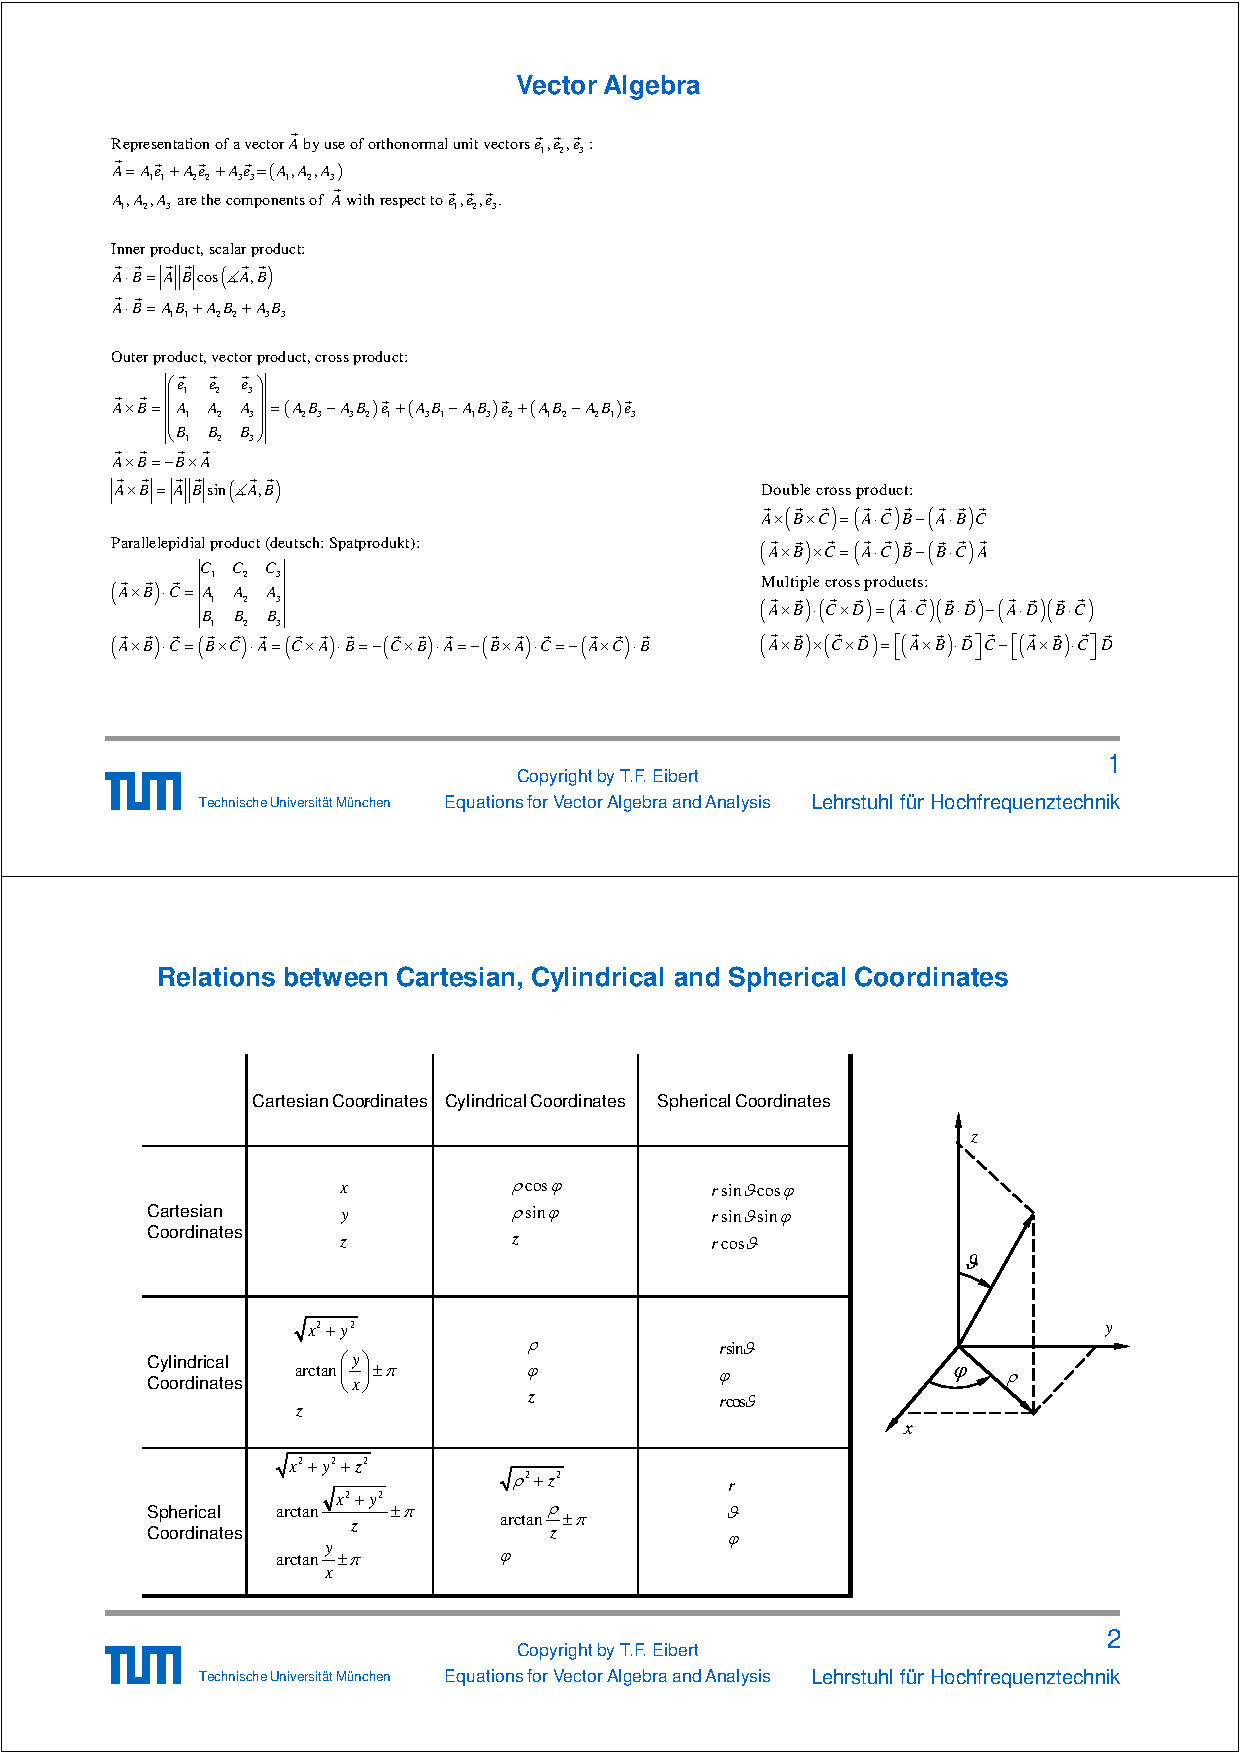
\includepdf[pages=-, nup=1x2, landscape=true]{extern/hf-vektor.pdf}% Vektoralgebra

%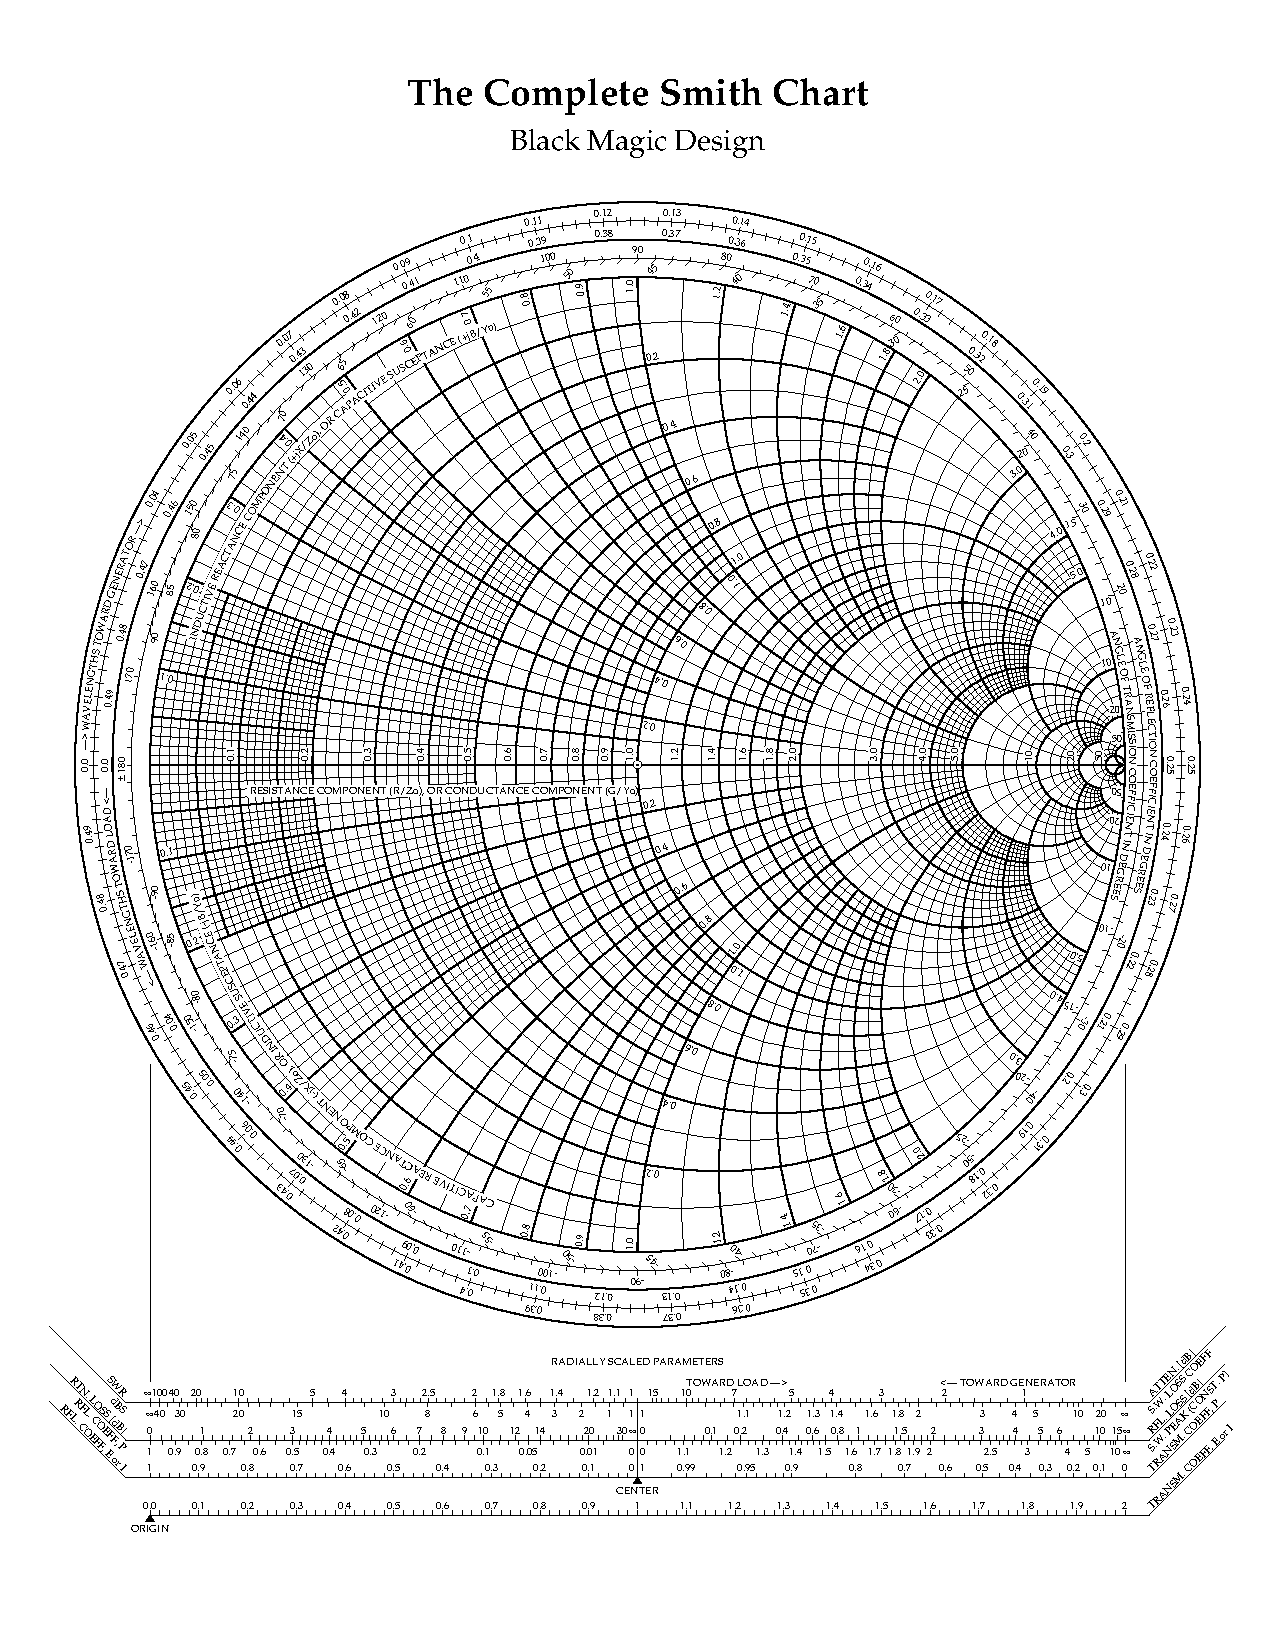
\includepdf[pages=-]{extern/smithchart.pdf}% Black Magic Smith Chart

\end{document}